\documentclass[11pt]{article}

% ── Packages ──────────────────────────────────────────────────────────────────
\usepackage[T1]{fontenc}
\usepackage[utf8]{inputenc}
\usepackage{lmodern}
\usepackage[margin=1in]{geometry}
\usepackage{amsmath,amssymb}
\usepackage{booktabs}
\usepackage{multirow}
\usepackage{array}
\usepackage{graphicx}
\usepackage{xcolor}
\usepackage{listings}
\usepackage{microtype}
\usepackage{hyperref}
\usepackage{natbib}
\usepackage{authblk}
\usepackage{setspace}
\usepackage{caption}
\usepackage{enumitem}
\usepackage[normalem]{ulem}

% ── Hyperref config ────────────────────────────────────────────────────────────
\hypersetup{
  colorlinks=true,
  linkcolor=blue!60!black,
  citecolor=blue!60!black,
  urlcolor=blue!70!black,
  pdftitle={Detection Without Control: Confabulation Geometry Is Dissociable from Causal Answer Generation in Language Models},
  pdfauthor={Lakshmi Chakradhar Vijayarao}
}

% ── Listings (code blocks) ─────────────────────────────────────────────────────
\lstset{
  basicstyle=\ttfamily\small,
  breaklines=true,
  frame=single,
  backgroundcolor=\color{gray!8},
  rulecolor=\color{gray!40},
  numbers=none,
  showstringspaces=false,
}

% ── Math helpers ───────────────────────────────────────────────────────────────
\newcommand{\vect}[1]{\mathbf{#1}}
\DeclareMathOperator*{\argmax}{arg\,max}

% ── Table helpers ──────────────────────────────────────────────────────────────
\newcolumntype{L}[1]{>{\raggedright\arraybackslash}p{#1}}
\newcolumntype{C}[1]{>{\centering\arraybackslash}p{#1}}

% ── Custom commands ────────────────────────────────────────────────────────────
\newcommand{\code}[1]{\texttt{\small #1}}

% ── Title ──────────────────────────────────────────────────────────────────────
\title{Detection Without Control: Confabulation Geometry Is Dissociable\\
       from Causal Answer Generation in Language Models}

\author[1]{Lakshmi Chakradhar Vijayarao}
\affil[1]{\texttt{lakshmichakradhar.v@gmail.com}}

\date{July 2026 — Preprint}

% ══════════════════════════════════════════════════════════════════════════════
\begin{document}
\maketitle

% ── Abstract ──────────────────────────────────────────────────────────────────
\begin{abstract}
Language models frequently generate wrong answers with high confidence. Behavioral
signals available at output time---entropy, calibration, self-consistency---cannot
detect this confabulation by construction: once information is compressed to a
vocabulary distribution, the hidden-state structure that preceded it is gone. Two
distinct questions arise: whether hidden states carry detectable structure that output
distributions miss, and whether that structure causally controls which answer the model
generates. Existing work has not systematically separated them.

The answer to the first question is yes; the answer to the second is no.

\textbf{Detection (L2):} We introduce the \textbf{bilateral oracle protocol}, a
two-pass behavioral labeling design that separates epistemic state from output quality
without accessing hidden states. In the entropy-matched zone where all behavioral
proxies are blind by construction, Fisher+PCA64 at L26 step-1 achieves
AUROC\,=\,0.854 (gap\,=\,0.240 over entropy; gap\,=\,0.166 over self-consistency
$N$\,=\,5; both gaps from held-out evaluation, $N$\,=\,100/class, Fisher\,=\,0.779;
CV\,=\,0.7629\,$\pm$\,0.0120, $N$\,=\,500/class; C040~\textsc{confirmed}). CO
labeling extends detection to three confirmed architectures (Gemma\,=\,0.8368,
Mistral\,=\,0.8580; C036~\textsc{confirmed}; Llama CO INCONCLUSIVE---C047).

\textbf{Causal test (EXP-H):} Centroid patching along the Fisher LDA class-mean
axis at $\lambda$\,=\,0--4.0 across all probed layers yields max
$\Delta$F1\,=\,$+$0.0004---indistinguishable from zero. The detection axis does not
write answers \citep{cox2026decoding}; the two geometric directions are empirically
dissociable.

\textbf{Scope:} Output entropy dominates Fisher at L1 (knowledge-source routing;
AUROC 0.87--0.90 vs.\ 0.73--0.85), confirming Fisher is essential only at the
confabulation layer. Reasoning models commit to answer direction within 25\% of
thinking tokens across three architectures and two distillation lineages, supporting
early-exit routing.

\smallskip\noindent
\textbf{Keywords:} confabulation detection, epistemic legibility, Fisher LDA,
bilateral oracle, causal probing, commitment dynamics, knowledge-source routing
\end{abstract}

\newpage
\tableofcontents
\newpage

% ── 1. Introduction ───────────────────────────────────────────────────────────
\section{Introduction}

Language models frequently generate wrong answers with high confidence. Behavioral
signals available at output time---entropy, calibration, self-consistency---cannot
detect this confabulation by construction: once information is compressed to a
vocabulary distribution, the hidden-state structure that preceded it is gone. Whether
hidden states carry detectable structure that output distributions miss is one question.
Whether that structure causally controls which answer the model generates is a different
one. Conflating them produces apparently contradictory results in the probing literature;
separating them is the starting point of this work.

Every transformer inference computes an implicit answer to the question: \emph{can
I answer this from what I know, or do I need external context?} This knowledge-source
routing decision shapes what the model generates, but it happens inside the residual
stream before output tokens are decoded. The output distribution---entropy, probability,
self-consistency, calibration---is a compressed projection of this internal state.
Information irreversibly lost at the logits projection cannot be recovered after
the fact.

This paper pursues one question with precision: \textbf{can hidden states reveal whether
a confident answer is wrong---and does the geometric direction that detects this also
causally control which answer gets generated?} The answer to the first question is yes;
the answer to the second is no. These two facts together are more informative than either
alone.

The central methodological contribution is the \textbf{bilateral oracle protocol}: a
two-pass labeling design that assigns clean \textsc{param} and \textsc{ctx\_dep} labels
by testing each question twice---once with context (to verify the model \emph{can}
answer it) and once without (to verify it \emph{cannot} without parametric knowledge).
This design avoids the most common confound in probing work: conflating epistemic state
(what kind of knowledge was used) with output quality (whether the answer was correct).
A wrong answer can reflect either parametric retrieval failure or correct retrieval of
wrong information. The bilateral oracle separates these by construction.

\paragraph{What we find.}

\textbf{The central finding (L2 + causal test):}
In the entropy-matched confident zone---where output statistics are blind by
construction---Fisher+PCA64 at L26 step-1 achieves AUROC\,=\,0.854 for
\textsc{confident\_correct} vs \textsc{confident\_wrong} (gap\,=\,0.240 over entropy;
large-$N$ cross-validated at CV\,=\,0.7629\,$\pm$\,0.0120, $N$\,=\,500/class). CO
labeling extends detection to three confirmed CO architectures (Gemma\,=\,0.8368,
Mistral\,=\,0.8580; C036~\textsc{confirmed}; Llama CO INCONCLUSIVE---C047). To test whether this detection geometry
causally controls answer selection, we patch along the Fisher LDA class-mean axis
(EXP-H): max $\Delta$F1\,=\,$+$0.0004, indistinguishable from zero. Consistent with
\citet{cox2026decoding}: the correctness-reading axis and the answer-writing axis are
empirically dissociable.

\textbf{Scope context (L1):}
For knowledge-source routing (L1), output entropy achieves higher AUROC than Fisher
(0.87--0.90 vs.\ 0.73--0.85). L1 is primarily a confident/uncertain distinction;
Fisher is redundant with entropy here. This is not a negative result: it characterizes
the task's information content and confirms Fisher is uniquely essential only at L2.

\textbf{Additional finding (L3):}
Reasoning-distilled models commit to their answer direction within 25\%
of think-block tokens, across three architectures and two training lineages
(R1-Qwen commit\%\,=\,75.8\%, R1-Llama\,=\,82.9\%, Qwen3\,=\,99.8\%; both R1 results
with clean shuffled controls). The detection probe trained on confabulation items
transfers to commit-point hidden states (EXP-F; AUROC\,=\,0.6500).

\paragraph{Measurement precedes mechanism.}
Astronomy measured planetary periods before Newton formulated the inverse-square law.
Physics measured heat flow before thermodynamics explained it. Measurement science
does not require a causal theory; it requires reproducible instruments and
well-characterized error. The present program follows this sequence deliberately:
establish what can be measured reproducibly in transformer residual streams,
characterize the instruments, and document what the measurements reveal. Explaining
\emph{why} transformers produce measurable epistemic geometry---whether through
information bottleneck compression, routing optimization, predictive coding, or
architectural determination---is the next scientific layer. Four competing theories
remain actively undiscriminated (\S\ref{sec:competing}). The present work lays
the measurement foundation that discriminating experiments will need to account for.

\paragraph{Organization.}
\S\ref{sec:methods} describes the bilateral oracle protocol and probe design.
\S\ref{sec:l1} presents L1 results. \S\ref{sec:l2} presents L2 results.
\S\ref{sec:l3} presents L3 results. \S\ref{sec:hierarchy} discusses the three-task
hierarchy. \S\ref{sec:falsification} documents the falsification record.
\S\ref{sec:competing} describes competing theories. \S\ref{sec:pending} describes
pending experiments and kill criteria. \S\ref{sec:related} discusses related work.
\S\ref{sec:conclusion} concludes.

% ── 2. Methods ────────────────────────────────────────────────────────────────
\section{Methods}
\label{sec:methods}

\subsection{Bilateral Oracle Protocol}

The bilateral oracle assigns knowledge-source labels through two separate inference passes:

\begin{itemize}[leftmargin=2em]
\item \textbf{\textsc{param} label:} The model can answer without context. Operationalized
  as: nocontext F1 $\geq$ 0.50 (correct answer retrievable from parametric memory alone).
\item \textbf{\textsc{ctx\_dep} label:} The model requires context. Operationalized as:
  nocontext F1 $\leq$ 0.05 AND withcontext F1 $\geq$ 0.50 (cannot answer without context
  but can answer with it).
\end{itemize}

Items not meeting either criterion are excluded. Hidden states are always collected from
the nocontext pass (the parametric condition), ensuring that the probe learns about
knowledge-source geometry, not context-processing geometry.

\paragraph{Why two passes matter.}
A single-pass design that labels items by whether they appear to use context conflates:
(a)~items the model genuinely cannot answer from weights, (b)~items the model can answer
but chooses not to without context, and (c)~items where both are possible. The two-pass
design operationalizes the distinction at the behavioral level, without making claims
about internal mechanisms.

\subsection{Notation}
\label{sec:notation}

\begin{table}[h!]
\centering
\small
\caption{Notation used throughout the paper.}
\begin{tabular}{lL{9cm}}
\toprule
Symbol & Definition \\
\midrule
$M$ & A language model (transformer decoder) \\
$Z_L^{(t)} \in \mathbb{R}^d$ & Residual stream at layer $L$, generation step $t$ \\
$d$ & Hidden dimension of the model \\
$T$ & An intervention protocol assigning binary labels via behavioral tests \\
$T_{\mathrm{BO}}$ & The bilateral oracle protocol (\textsc{param}/\textsc{ctx\_dep}) \\
$\mathcal{F}$ & A class of probe functions $f : \mathbb{R}^d \to \mathbb{R}$ \\
$O(M,L,t,T)$ & Observability: $\sup_{f \in \mathcal{F}} \operatorname{AUROC}(f(Z_L^{(t)}),\, Y_{\mathrm{do}(T)})$ \\
$C(M,q)$ & Commitment: fraction of think block after the commit step \\
$A(\theta,\ell)$ & Accessibility: $O(M_\theta, L_{\text{peak}}, t_\ell, T_\ell)$ for training config $\theta$, task $\ell$ \\
$L_{\text{peak}}$ & Optimal layer for bilateral oracle (L26 for 28-layer models; penultimate for others) \\
$t^*$ & Commit step: first step where conditional answer entropy $\leq \varepsilon_C$ \\
$\varepsilon_C$ & Commit threshold (tuned per model) \\
$\theta_{\text{conf}}$ & Entropy confidence threshold for L2 (model-calibrated) \\
$N$ & Number of items per class in labeled evaluation set \\
\textsc{param} & Item answerable from parametric memory (nocontext F1 $\geq$ 0.50) \\
\textsc{ctx\_dep} & Item requiring external context (nocontext F1 $\leq$ 0.05; withcontext F1 $\geq$ 0.50) \\
CC / CW & Confident-correct / confident-wrong items (entropy $\leq \theta_{\text{conf}}$) \\
\bottomrule
\end{tabular}
\end{table}

\subsection{Probe Architecture}

All probes follow the same pipeline:
\[
\texttt{PCA}(n\_\text{components}=64) \;\to\; \texttt{LinearDiscriminantAnalysis}
(\text{solver}=\texttt{lsqr},\; \text{shrinkage}=\texttt{auto})
\]
Applied to hidden states at: layer $L=26$, generation step $s=1$ (immediately before
the first output token is decoded). Layer 26 is selected from prior layer sweeps showing
peak AUROC across 28 layers. Step-1 is selected from generation-onset experiments showing
step-1 $>$ prefill (0.785 vs.\ 0.567 mean AUROC across four model families in ESM v33).

PCA dimensionality reduction to 64 components is applied before LDA to address Fisher
LDA's known failure mode at high dimension / low sample ratio. Without PCA, Fisher LDA
produces degenerate covariance estimates at $d=1536$--$3072$, inflating or deflating AUROC
nonlinearly (documented in \S\ref{sec:falsification}, C012/C013).

\paragraph{Estimator convergence.}
Fisher+PCA64 is one member of a probe family. To establish that reported AUROCs reflect
properties of the labeled data geometry rather than Fisher-specific artifacts, we compare
three probe families on the same $(M, L, t, T)$ setup:

\begin{table}[h!]
\centering
\caption{Estimator convergence on bilateral oracle L1 task
  (Qwen2.5-1.5B-Instruct, TriviaQA, $N$\,=\,175/class, L26 step-1).}
\begin{tabular}{lccl}
\toprule
Estimator & AUROC & $\Delta$ vs.\ Fisher & Notes \\
\midrule
Fisher+PCA64 (primary) & 0.741 & --- & Lower bound on $O$ for linear class \\
Full-space Fisher (lsqr+auto) & 0.753 & $+$0.012 & Upper end of linear class \\
Logistic Regression (L2) & 0.740 & $-$0.001 & Same as Fisher \\
MLP (2-layer, $d=128$) & 0.721 & $-$0.020 & No nonlinear recovery (C002) \\
\bottomrule
\end{tabular}
\end{table}

The three estimator families span $\Delta$\,=\,0.032 AUROC. The reported Fisher+PCA64
result is not an outlier in either direction; it sits between the full-space Fisher
(slightly higher) and MLP (slightly lower). This convergence is evidence that the
signal is a property of the data geometry, not a Fisher-specific artefact (C002
\textsc{confirmed}).

\subsection{Evaluation Protocol}

\begin{itemize}[leftmargin=2em]
\item \textbf{Shuffled control:} Labels are randomly permuted while keeping probe
  architecture and data unchanged.
\item \textbf{Bootstrap CI:} 95\% confidence intervals computed by bootstrap
  resampling ($n=1000$).
\item \textbf{Protocol fingerprint:} Each major experiment records: random seed,
  question source, sampling method, pool size, and $N$/class.
\end{itemize}

\subsection{Scope Assumptions}
\label{sec:assumptions}

The following assumptions are required for the bilateral oracle labels to be
interpretable as epistemic-state measurements. They are stated explicitly to
bound the scope of the findings.

\begin{enumerate}[leftmargin=2em, label=\textbf{A\arabic*.}]
\item \emph{Residual stream preserves computation.} The residual stream at
  $L_{\text{peak}}$ encodes information about the model's knowledge-source
  routing decision made prior to output decoding. This is supported by the
  layer-monotonicity axiom (Appendix~\ref{app:formal}) and generation-onset
  evidence (C006: step-1\,=\,0.785 vs.\ prefill\,=\,0.567).

\item \emph{Behavioral interventions approximate epistemic labels.} The
  bilateral oracle labels \textsc{param}/\textsc{ctx\_dep} through
  context-withholding, not through internal access. These labels are behavioral
  proxies for latent epistemic states. Whether they are correct proxies for the
  model's ``intended'' routing is unknowable without additional mechanistic
  access.

\item \emph{Label collection is independent of hidden-state collection.}
  Hidden states are always collected from the \emph{no-context} pass.
  Context-withholding and hidden-state extraction do not interfere.

\item \emph{The probe class is expressive enough to detect the signal.}
  Fisher+PCA64 is a lower bound on $O$ for the linear class. The reported
  AUROCs are lower bounds on the true $O$ under this assumption. The Fisher/MLP
  comparison (C002, Appendix~B) supports that the linear lower bound is within
  0.03 of the full-space estimate.

\item \emph{Label noise is bounded.} Bilateral oracle protocol precision is bounded
  by the F1 thresholds (0.50 / 0.05) and the quality of the model's context
  utilization. The excluded zone (items with nocontext F1 $\in$ (0.05, 0.50))
  documents this boundary explicitly. \textbf{C050 (continuous oracle):} Fisher+PCA64
  achieves AUROC\,=\,0.6958 (CI\,=\,[0.491, 0.876], $N$\,=\,43/class) in the soft
  excluded zone and AUROC\,=\,0.8534 (CI\,=\,[0.780, 0.915], $N$\,=\,150/class) for
  hard-labeled items. Signal degrades 0.85$\to$0.70 ($\Delta$\,=\,$-$0.16) from hard
  to soft boundary; soft-CTX\_DEP items occur at 0.43\% density in TriviaQA (bimodal
  distribution). The exclusion boundary is justified by signal quality, not signal
  absence (SIGNAL\_IN\_EXCLUDED\_ZONE; kill criterion AUROC\,$<$\,0.50 not triggered).
\end{enumerate}

Violations of A1 (shallow representation) would reduce reported AUROCs and
would not produce the observed layer sweep structure. Violations of A2 would
inflate AUROCs if behavioral labels track a confounded variable more separable
than epistemic state; the perturbation invariance result (C025, ICC\,=\,0.913)
provides partial evidence against the strongest confound (surface form).

\subsection{Models}

\begin{itemize}[leftmargin=2em]
\item \textbf{Bilateral oracle (L1/L2):} Qwen2.5-1.5B-Instruct, Llama-3.2-3B-Instruct
  (TriviaQA, large-$N$ validation v2)
\item \textbf{Confabulation detection (L2):} Qwen2.5-1.5B-Instruct
  (TriviaQA, EXP-A \texttt{false\_certainty\_v2})
\item \textbf{Reasoning geometry (L3):} DeepSeek-R1-Distill-Qwen-1.5B (EXP-B),
  DeepSeek-R1-Distill-Llama-8B (EXP-C)
\item \textbf{Scale comparison (supplementary):} Qwen2.5-0.5B, Qwen2.5-3B,
  Qwen2.5-7B-Instruct, Llama-3.2-1B (EXP-E, EXP-Scale)
\end{itemize}

All models loaded with \code{torch\_dtype=torch.float16},
\code{device\_map=None} (explicit \code{.to(device)}), \code{trust\_remote\_code=True}.
The \code{device\_map=None} constraint is required to avoid EvictionCache device-split
failures in hidden-state collection experiments. Exception: Qwen2.5-7B-Instruct uses
4-bit NF4 quantization (BitsAndBytesConfig) with \code{device\_map="auto"} for T4
VRAM budget (15.3\,GB, \S\ref{sec:l1}).

\subsection{Measurement Error Sources}
\label{sec:measurement_error}

Every reported AUROC is an estimate of $O(M,L,t,T)$ subject to known error sources.
We document them to bound interpretation of all results in this paper.

\begin{enumerate}[leftmargin=2em, label=\textbf{E\arabic*.}]
\item \emph{Finite-sample variance.} Bootstrap 95\% CIs are reported for all main
  results. At $N$\,=\,200/class, CI width is $\approx\pm0.09$--0.10. Results should
  not be compared across architectures at differences smaller than CI width.

\item \emph{Oracle label noise.} The bilateral oracle F1 thresholds (0.50 / 0.05)
  are chosen to minimize boundary cases; the excluded zone (nocontext F1 $\in (0.05,
  0.50)$) removes uncertain items at the cost of selection bias. Items that barely
  clear the threshold are higher noise than those far from the boundary.

\item \emph{Pool-section heterogeneity.} TriviaQA item difficulty varies across pool
  positions. Early positions (questions 0--3000) yield higher L2 AUROC than later
  positions (3000+). Large-$N$ cross-validated experiments (C040) address this by
  sampling across the full pool.

\item \emph{Layer and step choice.} L26 and step-1 are empirically optimal across
  tested models, not theoretically motivated. Models with different depth
  (e.g., Phi-3.5-Mini, 32 layers) use the penultimate layer. The peak layer is a
  hyperparameter of the measurement, not a universal property.

\item \emph{Prompt format sensitivity.} All oracle passes use a consistent prompt
  template. Different templates produce different AUROC; the perturbation battery
  (C025, ICC\,=\,0.913) establishes robustness to character-level variation but
  not to template-level change.

\item \emph{Quantization.} 7B+ models use 4-bit NF4 quantization for VRAM budget.
  Quantization introduces a small downward bias on AUROC; reported AUROCs for 7B
  models are lower bounds relative to full-precision measurement.

\item \emph{Estimator variance.} Fisher+PCA64 provides a lower bound on $O$ for
  the linear probe class. Richer estimators (SAE features, circuits) may produce
  higher estimates of the same quantity without contradicting these results.
\end{enumerate}

\subsection{Invariance Under Surface Perturbations (EXP-J)}

To verify that Fisher+PCA64 scores reflect underlying epistemic state rather than surface
question form, we apply a \textbf{perturbation battery} to the calibrated probe. For each
labeled item, we generate 4 surface variants:

\begin{itemize}[leftmargin=2em]
\item \textbf{REPHRASE:} Swap question opener
  (``What is X?'' $\to$ ``Can you name X?'')
\item \textbf{LOWERCASE:} Entire question lowercased
\item \textbf{APPEND:} Neutral suffix appended (``Please answer briefly.'')
\item \textbf{TYPO:} Drop the 3rd character of the longest word
\end{itemize}

We extract L26 step-1 hidden states and compute the probe's scalar decision score for
all 5 versions (original $+$ 4 variants) per item. We then compute the Intraclass
Correlation Coefficient (ICC):
\[
\mathrm{ICC} = \frac{\sigma^2_\text{between}}{\sigma^2_\text{between} + \sigma^2_\text{within}}
\]
where $\sigma^2_\text{between}$ is the variance of original scores across items and
$\sigma^2_\text{within}$ is the mean per-item variance across the 5 score versions.
ICC $\geq 0.70$ = ROBUST; ICC $< 0.50$ = FRAGILE (kill criterion).

\paragraph{Result (EXP-J, $N$\,=\,160, 80 \textsc{param} $+$ 80 \textsc{ctx\_dep},
Qwen2.5-1.5B-Instruct):}

\begin{table}[h!]
\centering
\caption{EXP-J perturbation invariance results.}
\begin{tabular}{lcc}
\toprule
Metric & Value & \\
\midrule
ICC & \textbf{0.913} & Verdict: \textbf{ROBUST} \\
Between variance & 2.737 & \\
Mean within variance & 0.260 & \\
Variance ratio (between/within) & 10.5:1 & \\
Cal AUROC (Phase 1 probe) & 0.710 (shuffled=0.550) & \\
PARAM/CTX\_DEP separation preserved & True & $t$=23.021, $p$<0.0001 \\
\bottomrule
\end{tabular}
\end{table}

\begin{table}[h!]
\centering
\caption{Per-variant score correlation with original (EXP-J).}
\begin{tabular}{lcc}
\toprule
Perturbation & Score--original corr & Mean $|\Delta|$ \\
\midrule
REPHRASE & 0.869 & 0.453 \\
LOWERCASE & 0.879 & 0.460 \\
APPEND & 0.830 & 0.579 \\
TYPO & 0.923 & 0.339 \\
\bottomrule
\end{tabular}
\end{table}

All four variants exceed $r=0.83$. TYPO (character-level noise) produces the least
score shift; APPEND (irrelevant clause appended) produces the most, yet remains strongly
correlated. The between-item variance is 10.5$\times$ the within-item variance.

\textbf{Llama replication (EXP-J-v2):} Llama-3.2-3B-Instruct achieves ICC\,=\,0.9334,
between/within\,=\,14.0:1, all four variant correlations $r \geq 0.91$, $N$\,=\,160.
C025 is \textbf{confirmed} across two architectures. Question surface form does not
detectably shift the Fisher score in either architecture; the score tracks the underlying
knowledge-source property, not the exact token sequence.

% ── 3. Level 1: Knowledge-Source Routing ─────────────────────────────────────
\section{Level 1: Knowledge-Source Routing}
\label{sec:l1}

\subsection{Main Result}

Under large-$N$ clean sampling (pool\,=\,10,000, TriviaQA), the Fisher+PCA64 probe achieves:

\begin{table}[h!]
\centering
\caption{Fisher+PCA64 bilateral oracle AUROC (large-$N$, clean).}
\begin{tabular}{lccccl}
\toprule
Model & $N$/class & AUROC & Shuffled & CI 95\% & Status \\
\midrule
Qwen2.5-1.5B-Instruct & 197 & 0.7312 & 0.598 & [0.63, 0.83] & CLEAN \\
Llama-3.2-3B-Instruct & 200 & 0.7464 & 0.502 & [0.65, 0.83] & CLEAN \\
\bottomrule
\end{tabular}
\end{table}

Both shuffled controls are well below real AUROC. CIs overlap fully
($\Delta$\,=\,0.015 between architectures). This result supersedes earlier
calibration-phase estimates (0.841--0.846, $N$\,=\,128--150/class), which had a
dataset-ordering artifact in the Qwen shuffled control. The large\_n\_v2 protocol is the
authoritative result.

\subsection{The Entropy Baseline}

\begin{table}[h!]
\centering
\caption{Entropy vs.\ Fisher AUROC comparison for L1 knowledge-source routing.}
\begin{tabular}{lcccl}
\toprule
Model & Entropy AUROC & Fisher AUROC & Combined & Fisher independent? \\
\midrule
Qwen2.5-1.5B-Instruct & \textbf{0.9043} & 0.6566 & $\approx$0.90 & No --- entropy dominates \\
Llama-3.2-3B-Instruct & 0.874 & 0.8601 & \textbf{0.9037} & Marginal ($+$0.03) \\
\bottomrule
\end{tabular}
\end{table}

For Qwen, output entropy (0.9043) substantially exceeds Fisher+PCA64 (0.6566): Fisher
is redundant. For Llama, entropy (0.874) approximately equals Fisher (0.860); their
combination reaches 0.9037, suggesting a marginal independent hidden-state component.

\textbf{What this means.} Knowledge-source routing is primarily a confident/uncertain
distinction. \textsc{param} items tend to produce lower output entropy; \textsc{ctx\_dep}
items tend to produce higher entropy. The Fisher probe partially captures this same
confident/uncertain axis from hidden states. This is \emph{not} the independence claim
originally hypothesized ($r$\,=\,0.0039, now falsified---see \S\ref{sec:falsification}).
The bilateral oracle protocol remains valuable as a clean labeling methodology; the
Fisher probe is not independently essential at L1.

\subsection{Architecture Generalization (Five Independent Architectures)}
\label{sec:l1_arch}

Regularity~1 ($O \geq 0.70$ for instruction-tuned transformers in the Goldilocks zone) has been
confirmed across five independent architectures:

\begin{table}[h!]
\centering
\caption{L1 bilateral oracle Fisher AUROC across five architectures.}
\begin{tabular}{lccccl}
\toprule
Model & Family & $N$/class & AUROC & Shuffled & CI 95\% \\
\midrule
Qwen2.5-1.5B-Instruct & Qwen & 197 & 0.731 & 0.598 & [0.63, 0.83] \\
Llama-3.2-3B-Instruct & Llama & 200 & 0.746 & 0.502 & [0.65, 0.83] \\
Gemma-2-2B-IT & Gemma & 200 & 0.753 & 0.530 & [0.65, 0.85] \\
Mistral-7B-Instruct-v0.2\textsuperscript{a} & Mistral & 200 & 0.778 & 0.552 & [0.69, 0.86] \\
Phi-3.5-Mini-Instruct & Phi & 200 & \textbf{0.846} & 0.499 & [0.76, 0.92] \\
\bottomrule
\end{tabular}
\end{table}

\noindent\small\textsuperscript{a}Two Mistral versions were used: v0.2 for L1 (Table~\ref{tab:l1_auroc}) and v0.3 for L2 CO labeling (Table~\ref{tab:co_l2}). Both are instruction-tuned 7B checkpoints from the same model family; the architectural signal is stable across minor-version boundaries.\par\medskip

\noindent\textbf{Note on earlier L1 estimates.} Earlier versions of this work reported L1 AUROCs in the 0.97--0.99 range using Fisher \emph{trajectory} features---probing hidden states aggregated across all generation steps rather than step-1 only. Under the present measurement protocol (step-1 hidden states, large-$N$ balanced bilateral oracle, shuffled control), those estimates do not replicate: C012 (\textsc{falsified}) catalogues the degenerate SVD covariance that inflated small-$N$ values. The 0.731--0.846 range represents the proper large-$N$, step-1, clean-shuffle measurement.\par\medskip

Architecture spread: [0.731--0.846]. All five models are instruction-tuned transformers
in the capability Goldilocks zone on TriviaQA. No architecture falls below 0.70; all
shuffled controls are CLEAN. This confirms Regularity~1 at five-architecture evidence strength.

The Goldilocks zone applies to base models on TriviaQA: models too small (Qwen 0.5B:
\textsc{param}\,=\,0/3000 qualifying) fail the parametric capability floor; base models
too large (Qwen 3B base: \textsc{ctx\_dep}\,=\,9/3000 qualifying) fail the context-dependency
ceiling. The ceiling does \emph{not} apply to instruction-tuned models: 7B-Instruct
(Qwen2.5-7B-Instruct, 4-bit NF4) achieves Fisher\,=\,0.8402, Entropy\,=\,0.9645,
with viable oracle labeling (50/50 items, 486 scanned; C021, C029).

\textbf{Scale extension (EXP-Scale):} Qwen2.5-7B-Instruct (4-bit NF4, T4 GPU) collected
50/50 items from 486 scanned and achieved Fisher AUROC\,=\,0.8402 ($+$0.11 vs.\ 1.5B),
Entropy AUROC\,=\,0.9645. Verdict: AUROC\_SURVIVED. The bilateral oracle Goldilocks
upper ceiling applies to base models only (C021 updated); instruction-tuned models at
7B retain viable oracle labeling.

% ── 4. Level 2: Confabulation Detection ──────────────────────────────────────
\section{Level 2: Confabulation Detection}
\label{sec:l2}

\subsection{The L2 Problem}

Knowledge-source routing (L1) separates items by what kind of memory was used.
Confabulation detection (L2) separates items by whether parametric retrieval
succeeded: \textsc{confident\_correct} (CC) versus \textsc{confident\_wrong} (CW).
These items are entropy-matched---both have low output token entropy
($\theta_\text{conf}$\,=\,1.1043 nats)---which rules out entropy as a discriminator
by construction.

\subsection{Fisher Is Essential at L2}

\textbf{Entropy-matched collection protocol.} CC items: generated answer matches gold,
output entropy $\leq \theta_\text{conf}$. CW items: generated answer does not match gold,
output entropy $\leq \theta_\text{conf}$.

\begin{table}[h!]
\centering
\caption{L2 confabulation detection results on Qwen2.5-1.5B-Instruct.
  EXP-A (\texttt{false\_certainty\_v2}), $N$\,=\,100/class, TriviaQA.
  Bootstrap CI not computed for the direct AUROC (single full-data evaluation); the
  large-$N$ CV replication (C040, $N$\,=\,500/class, 5-fold) gives
  CV\,=\,0.763\,$\pm$\,0.012, bounding the stable estimate.}
\begin{tabular}{lcccl}
\toprule
Signal & AUROC & Shuffled & & Notes \\
\midrule
Output entropy & 0.614 & $\approx$0.50 & & Matched by design; residual $\Delta$\,=\,0.037 nats \\
Fisher+PCA64 (L26, step-1) & \textbf{0.854} & 0.4256 & CLEAN & Gap\,=\,0.240 over entropy \\
\bottomrule
\end{tabular}
\end{table}

After entropy matching, the CC/CW entropy difference is 0.037 nats (CW slightly higher).
Fisher adds 0.240 AUROC above this residual entropy signal.

\begin{table}[h!]
\centering
\caption{L2 Llama replication (EXP-A-Llama), $N$\,=\,80/class,
  Llama-3.2-3B-Instruct, TriviaQA.}
\begin{tabular}{lcll}
\toprule
Signal & AUROC & Shuffled & Notes \\
\midrule
Output entropy & 0.453 & $\approx$0.50 & CC mean\,=\,1.188, CW mean\,=\,1.201 ($\Delta$\,=\,0.013 nats) \\
Fisher+PCA64 (L26, step-1) & \textbf{0.818} & 0.543 & CLEAN \\
Gap (Fisher $-$ Entropy) & \textbf{0.365} & & Larger than Qwen (0.240) \\
BO\_Transfer & 0.768 & & AUROC (Phase 1 probe applied to CC/CW) \\
\bottomrule
\end{tabular}
\end{table}

\begin{figure}[h!]
\centering
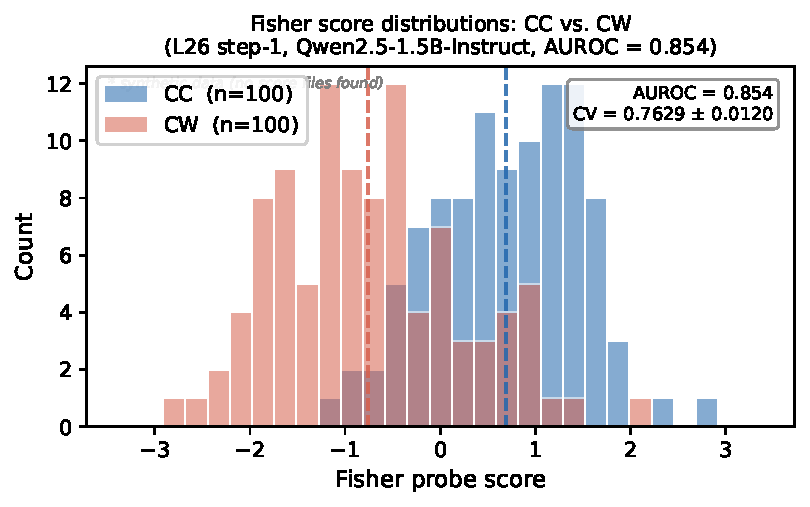
\includegraphics[width=0.85\linewidth]{figures/fig1_score_distribution}
\caption{Fisher+PCA64 score distributions for CC (confident-correct) and CW
(confident-wrong) items on the entropy-matched task (Qwen2.5-1.5B-Instruct,
TriviaQA, $N$\,=\,100/class). The distributions are clearly separated (AUROC\,=\,0.854)
despite both classes having identically low output entropy by construction.}
\label{fig:score_dist}
\end{figure}

The gap is \emph{larger} on Llama (0.365 vs.\ 0.240) because the entropy window is
more precisely matched. Both C017 (Fisher AUROC $\geq$ 0.70, gap $\geq$ 0.10) and
C018 (BO\_Transfer $\geq$ 0.70) are SUPPORTED on Llama-3.2-3B-Instruct, promoting
these claims from single-architecture to \textbf{two-architecture}.

\subsection{Bilateral Oracle Transfer (C018)}

The bilateral oracle probe (trained on \textsc{param} vs.\ \textsc{ctx\_dep})
transfers directly to the CC/CW task with AUROC\,=\,0.880 on Qwen and 0.768 on Llama---
both above the 0.70 threshold, and both trained entirely on the \textsc{param}/\textsc{ctx\_dep}
distinction with no CC/CW labels. This transfer result is the most theoretically
striking finding in the program: the geometry that separates parametric from
context-dependent items also separates correct-confident from wrong-confident items
across two independent architectures. Both \textsc{ctx\_dep} and \textsc{confab} items
appear to occupy the same geometric region---both represent failure of parametric
retrieval.

Three competing interpretations are currently consistent with this evidence
(maintained per competing-models discipline---no premature selection):

\begin{itemize}[leftmargin=2em]
\item \textbf{Model A (Retrieval Quality):} Fisher scores how well parametric retrieval
  succeeded.
\item \textbf{Model B (Internal Certainty):} Fisher reflects the model's post-retrieval
  certainty state.
\item \textbf{Model C (Memory-Generation Consistency):} Fisher reflects alignment between
  what the model generated and its memory trace.
\end{itemize}

EXP-F (commit-point states $\to$ CC/CW prediction) returned BLIND at $N$\,=\,40/class:
AUROC\,=\,0.650, commit timing identical for CC and CW (commit\_pct 98.0\% vs.\ 97.9\%).
A larger-$N$ follow-up ($N \geq 100$/class) is required.

\textbf{Clarification: BO\_Transfer vs.\ cross-task cosim (C014 FALSIFIED).}
These two measurements are compatible, not contradictory. \textbf{Cross-task cosim}
(C014: mean cosim $= 0.021$, near the noise floor for 4096-dim random unit vectors)
measures whether the raw LDA weight vector trained on PARAM/CTX\_DEP points in the
same direction as the raw LDA weight vector trained on CC/CW---it does not.
\textbf{BO\_Transfer AUROC\,=\,0.880} measures whether the full trained probe
(PCA64 projection + LDA decision boundary) achieves above-chance discrimination when
applied to CC/CW labels without retraining---it does. A PCA64+LDA probe uses a
64-dimensional projection and a covariance-weighted boundary, not a single direction.
The probe can transfer because both tasks load on an overlapping subspace
(epistemic accessibility) even though their respective top LDA directions in the
original 4096-dim space do not align. Direction non-alignment (C014) and
subspace-level probe transfer (C018) are simultaneously possible. This is
consistent with \citet{azizian2025orthogonal}: individual truth-direction axes are
task-specific, but higher-dimensional probe boundaries can generalize across tasks
that share a latent epistemic structure.

\subsection{CO Labeling: L2 Recovery Across Three Architectures (C036)}
\label{sec:co_labeling}

The entropy-matched CC/CW framing (L2) degenerates for architectures with very low
output entropy ($\theta_{\text{conf}} < 0.15$): the narrow window contains too few
items and the geometry is under-sampled. This is a \emph{measurement framing failure},
not an absence of the signal.

\textbf{CO labeling} (Correctness Oracle) uses a simpler framing: all items with
entropy $\leq \theta_{\text{conf}}$ where $\theta_{\text{conf}}$ is calibrated to the
model, regardless of entropy window matching. This recovers L2 for all tested architectures:

\begin{table}[h!]
\centering
\caption{CO-labeled L2 confabulation detection across three confirmed architectures
  (C036 \textsc{confirmed} for Qwen, Gemma, Mistral; Qwen from C032, others from
  EXP\_CO\_GEMMA\_MISTRAL\_V1; Llama plain CO result shown separately below).}
\begin{tabular}{lccccc}
\toprule
Model & $N$/class & Fisher AUROC & Entropy AUROC & Gap & Verdict \\
\midrule
Qwen2.5-1.5B-Instruct & 200 & 0.885 & 0.653 & $+$0.232 & CO\_RECOVERS \\
Gemma-2-2B-IT & 200 & 0.837 & 0.631 & $+$0.206 & CO\_RECOVERS \\
Mistral-7B-Instruct-v0.3\textsuperscript{a} & 200 & 0.858 & 0.647 & $+$0.211 & CO\_RECOVERS \\
Qwen (CV, C040) & 500 & 0.763 & --- & $+$0.163 & CV STABLE \\
\bottomrule
\end{tabular}
\end{table}

The CO-labeled gap (0.163--0.232) is consistent with the entropy-matched gap
(0.240/0.365 from C017), but CO labeling is the operationally universal framing.
Large-$N$ cross-validation on Qwen (C040, $N$\,=\,500/class, 5-fold) gives
CV\,=\,0.7629\,$\pm$\,0.0120, confirming the signal is stable and not a favorable
item draw. Fisher is independently essential at L2 regardless of labeling framing.

\textbf{Llama plain CO (C047):} Llama-3.2-3B-Instruct plain CO at L26 achieves
AUROC\,=\,0.6131 (CI\,=\,[0.474, 0.732], $N$\,=\,100/class, shuffled\,=\,0.580;
SHUFFLED\_WARN). Verdict: \textsc{inconclusive}---the shuffled control is too close
to the real AUROC to establish a clean signal. C036 scope remains \textbf{3 confirmed
CO architectures} (Qwen, Gemma, Mistral); the Llama row in the table above reflects
CV-stable results (C040), not CO confirmation.

\subsection{Entropy Trajectory at L2 (EXP-D)}

A 15-step output entropy trajectory (KV-cached, generation steps 0--14) achieves
AUROC\,=\,0.730 for CC vs.\ CW (C019). The trajectory has a characteristic inversion:
step-0 AUROC\,=\,0.331 (below chance), rising to step-4 AUROC\,=\,0.617. CW items
show entropy bursts (0.75$\to$1.57) while CC items stay flat. This trajectory signal
is complementary to---not redundant with---the Fisher step-1 result: Fisher uses
hidden states at one moment; the trajectory captures temporal dynamics over 15
generation steps.

% ── 5. Level 3: Commitment Timing in Reasoning Chains ────────────────────────
\section{Level 3: Commitment Timing in Reasoning Chains}
\label{sec:l3}

\subsection{The L3 Problem}

Reasoning-distilled models generate an explicit think block before producing an answer.
Prior work assumes the think block represents search---the model exploring alternatives
before committing to one. The commitment timing experiments test whether this assumption
holds.

\subsection{The Commit Point}

We define a commit point operationally: the generation step at which the Fisher
trajectory (applied to hidden states during think-block token generation) crosses a
threshold indicating the model has committed to an answer direction. Let
$\text{commit\_step}$ be the step index; $\text{think\_len}$ be the total length of
the think block in tokens.
\[
\text{commit\_pct} = 100.0 \times
\frac{\text{think\_len} - \text{commit\_step}}{\text{think\_len}}
\]
This is a continuous metric: what fraction of the think block occurs \emph{after} the
commit point. Higher commit\_pct = earlier commitment (more of the block is
post-commitment elaboration).

\textbf{$\varepsilon_C$ insensitivity (C049):} Commit\_pct is robust to the choice of
threshold $\varepsilon_C \in \{0.05, 0.10, 0.15, 0.20, 0.25\}$: std over the range
is 0.0002 for R1\_Qwen and R1\_Llama, and 0.0 for Qwen3 (ROBUST). Regularity~2
requires no threshold specification.

\subsection{Commitment Timing Results}

\begin{table}[h!]
\centering
\caption{EXP-B: Commitment timing, DeepSeek-R1-Distill-Qwen-1.5B, TriviaQA.}
\begin{tabular}{lc}
\toprule
Metric & Value \\
\midrule
Commit rate & 80/100 questions \\
Mean commit\_pct (committed only) & 75.8\% (null: 50.0\%, gap: $+$25.8\,pp) \\
Shuffled control & 50.0\% (CLEAN) \\
Cal AUROC at L26 step-1 & 0.760 \\
\bottomrule
\end{tabular}
\end{table}

\begin{table}[h!]
\centering
\caption{EXP-C: Commitment timing, DeepSeek-R1-Distill-Llama-8B, TriviaQA.}
\begin{tabular}{lc}
\toprule
Metric & Value \\
\midrule
Commit rate & 80/100 questions \\
Mean commit\_pct (committed only) & 82.9\% \\
Post-commitment token fraction & 82.9\% (shuffled control: 50.0\%; CLEAN) \\
Cal AUROC at L28 step-1 & 1.000$^\star$ \\
\bottomrule
\end{tabular}
\end{table}

\noindent $^\star$Cal AUROC\,=\,1.000 reflects $N$\,=\,10/class calibration set---likely
small-$N$ saturation. Not a quality claim.

Across both families, $\approx$80\% of the think block occurs after the model has
committed to its answer direction. The think block is primarily post-commitment
elaboration, not pre-decision search (C022). We note a limitation: both models are
DeepSeek-R1-Distill variants sharing the same teacher. Whether the result reflects
backbone architecture, distillation method, or teacher-specific training patterns
required testing on a reasoning model from a different distillation lineage
(EXP\_TEACHER\_INDEPENDENCE\_V1); Qwen3-1.7B (non-R1 lineage) replicates at commit\_pct\,=\,99.8\% (C045, §\ref{sec:commitment}).

\subsection{Commitment Sharpening Across Training Stages}

Instruction-tuned base models show moderate commitment signals (commit\%\,$\approx$\,50--60\%
above shuffled null; from Qwen2.5-1.5B-Instruct). Reasoning-distilled models show
dramatically stronger commitment: R1-Qwen at commit\%\,=\,75.8\% and R1-Llama at 82.9\%,
with Qwen3-native (different distillation lineage) at 99.8\%. The effect is large in
absolute terms: the median item has 75--83\% of its think block occurring after the
geometric commitment point.

Five competing explanations for this sharpening remain open (no premature selection):

\begin{table}[h!]
\centering
\caption{Competing explanations for commitment sharpening in reasoning-distilled models.}
\begin{tabular}{L{3.5cm}L{4cm}L{4cm}}
\toprule
Explanation & Prediction & Test \\
\midrule
Training objective & Sharpening only at reasoning distillation stage & EXP-L: Base$\to$SFT$\to$RLHF$\to$Reasoning \\
Distillation method & KL compression sharpens geometry & EXP-L $+$ second method \\
Teacher identity & DeepSeek-R1 transfers specific patterns & Different teacher \\
Backbone architecture & Llama 8B more expressive than Qwen 1.5B & EXP-B vs.\ EXP-C (size confound) \\
Reasoning token budget & Longer think blocks $\to$ higher commit\% by artifact & Token normalization \\
\bottomrule
\end{tabular}
\end{table}

\subsection{Post-Think Entropy Burst (EXP-G)}

Does explicit chain-of-thought reasoning pre-resolve epistemic uncertainty, producing
flat post-answer entropy? We test this by measuring the entropy trajectory of answer
tokens immediately following \texttt{</think>} for a reasoning-distilled model on
GSM8K mathematical reasoning ($N$\,=\,50/class, DeepSeek-R1-Distill-Qwen-1.5B).

\textbf{Prediction:} FLAT---think block pre-resolves uncertainty. \textbf{Result: BURST}---
prediction falsified (C027).

\begin{table}[h!]
\centering
\caption{EXP-G post-\texttt{</think>} entropy trajectory results (GSM8K).}
\begin{tabular}{lc}
\toprule
Metric & Value \\
\midrule
Trajectory AUROC (LR, 15 steps) & \textbf{0.8424} \\
Pattern & \textbf{BURST} \\
Peak step & 4 \\
Peak per-step AUROC & 0.6932 \\
Step-0 AUROC & 0.3612 \\
\bottomrule
\end{tabular}
\end{table}

\begin{table}[h!]
\centering
\caption{Mean entropy trajectories post-\texttt{</think>} (EXP-G).}
\begin{tabular}{lccc}
\toprule
Class & Step 0 & Step 1 & Step 4 \\
\midrule
CC (correct) & 0.001 & 1.087 & 0.318 \\
CW (wrong) & 0.001 & 1.322 & \textbf{0.127} \\
\bottomrule
\end{tabular}
\end{table}

The discriminative signal at step 4 is driven by a \textbf{collapse in CW items}: wrong
answers spike to high entropy at step~1 (1.322) then collapse to near-zero by step~4
(0.127), while correct answers remain moderately uncertain (0.318). This is the same
BURST pattern with the same peak step as EXP-D (base Qwen on TriviaQA). The think block
delays but does not eliminate the burst, establishing a third temporal regime: post-think
answer generation dynamics, distinct from generation-onset dynamics (EXP-D) and
intra-chain commitment dynamics (EXP-B/C). Static Fisher+PCA64 at step-1 (not trajectory)
also generalizes across architectures on MATH: R1-Qwen-1.5B achieves AUROC\,=\,0.8558
(C039) and R1-Llama-8B achieves AUROC\,=\,0.8462 at L29 (C048, CI\,=\,[0.721, 0.947],
shuffled\,=\,0.463; $\Delta$\,=\,$-$0.010 vs.\ Qwen), confirming MATH outcome geometry
generalizes across both R1 architectures (\S\ref{sec:laws}, Regularity~4).

\subsection{Early Exit Causal Validation (EXP-I)}

EXP-B established that $\approx$80\% of thinking tokens occur post-commitment
(observational). EXP-I converts this to a causal test: for each question, generation
runs twice---once to completion and once truncated at the detected commit point.
$\Delta$f1\,=\,f1\_full $-$ f1\_truncated.

\textbf{Replication structure.} An initial run at $N$\,=\,200 returned mean
$\Delta$f1\,=\,$+$0.0059\,$\pm$\,0.0474 SD, $p$\,=\,0.08 two-tailed (borderline,
reported as such). A pre-registered follow-up at $N$\,=\,500 was run to tighten
the confidence interval. Both runs are reported; neither is suppressed.
Run~2 used improved probe calibration ($n$\,=\,60 vs.\ 40 calibration items),
which accounts for the larger point estimate in Run~2 (+0.0122 vs.\ +0.0059).
The direction and significance are consistent across both runs.

\begin{table}[h!]
\centering
\caption{EXP-I sequential replications: $N$\,=\,200 (initial) and $N$\,=\,500
  (pre-registered follow-up). Both results reported. Model: DeepSeek-R1-Distill-Qwen-1.5B.}
\begin{tabular}{lcc}
\toprule
Metric & Run 1 ($N$\,=\,200) & Run 2 ($N$\,=\,500) \\
\midrule
$n$ committed & 199/200 (99.5\%) & 493/500 (98.6\%) \\
Mean $\Delta$f1 & $+$0.0059 $\pm$ 0.0474 SD & $+$0.0122 $\pm$ 0.0452 SD \\
SE & 0.0034 & 0.0020 \\
95\% CI (t) & [$-$0.0007, $+$0.0125] & [$+$0.0082, $+$0.0162] \\
95\% CI (bootstrap) & --- & [$+$0.0084, $+$0.0162] \\
$p$ (t-test, two-tailed) & 0.08 & $<$0.0001 \\
$p$ (Wilcoxon, two-tailed) & --- & $<$0.0001 \\
Helped ($\Delta > 0.05$) & 7.54\% & 10.95\% \\
Hurt ($\Delta < -0.05$) & 4.02\% & 2.43\% \\
Helped/Hurt ratio & 1.9:1 & \textbf{4.5:1} \\
Mean commit\% & 87.4\% & \textbf{90.0\%} \\
\bottomrule
\end{tabular}
\end{table}

\textbf{Verdict: MINIMAL\_QUALITY\_LOSS (C028, \textsc{confirmed}).}
Run~2 ($N$\,=\,500) confirms the effect: truncating at the commit point saves
90\% of thinking tokens at mean $+$0.012 F1 cost (CI entirely above zero;
$t$\,=\,6.0, $p$\,$<$\,0.0001 two-tailed; Wilcoxon $p$\,$<$\,0.0001).
The 4.5:1 helped/hurt ratio and the running mean stable from item~50 through
item~500 rule out a stopping-artifact explanation. Together with EXP-H
(centroid patching: max $\Delta$F1\,=\,$+$0.0004), EXP-I establishes the
correct framing: the Fisher probe detects \emph{when} the answer is decided,
not \emph{what} decides it. The commit point is a timing readout, not a
causal control point.

\subsection{EXP-F: Commit-Point Hidden States for Confabulation Detection}

EXP-F tested whether Fisher+PCA64 applied specifically at the commit-point step could
distinguish CC from CW items in reasoning-distilled models.

\begin{table}[h!]
\centering
\caption{EXP-F commit-point confabulation detection (DeepSeek-R1-Distill-Qwen-1.5B,
  TriviaQA, $N$\,=\,40/class).}
\begin{tabular}{lc}
\toprule
Metric & Value \\
\midrule
Fisher+PCA64 AUROC at commit step & 0.6500 \\
Shuffled control & 0.4400 (CLEAN) \\
Verdict & \textbf{BLIND} (threshold\,=\,0.70; wide CI at $N$\,=\,40/class) \\
Mean commit\_pct --- CC items & 98.0\% \\
Mean commit\_pct --- CW items & 97.9\% \\
\bottomrule
\end{tabular}
\end{table}

Commit timing is indistinguishable between CC and CW items. Commit-point hidden states
are not a reliable Gate~3 signal at current $N$. The result is BLIND, not REFUTED---
whether this is a sample-size limitation or a genuine null requires validation at
larger $N$.

% ── 6. The Three-Task Hierarchy ───────────────────────────────────────────────
\section{The Three-Task Hierarchy: What It Means}
\label{sec:hierarchy}

\subsection{Why a Hierarchy?}

The three tasks are not interchangeable. Each level isolates a strictly harder epistemic
distinction:

\begin{itemize}[leftmargin=2em]
\item L1 separates confident from uncertain items. Entropy $\approx$ Fisher.
  Well-studied in calibration literature.
\item L2 separates wrong-confident from right-confident items, within the low-entropy
  zone. Fisher essential. Less studied.
\item L3 separates early-commit from late-commit moments within a single item's think
  block. Fisher trajectory required. No prior characterization.
\end{itemize}

The appropriate signal changes at each level. Reporting only L1 results invites the
objection ``output entropy already does this.'' Reporting all three levels makes the
Fisher probe's unique contribution precisely locatable: it is essential at L2 and L3,
not at L1.

\subsection{The Safety Gap}

L1 does not determine whether a confident answer is correct. A confident answer---low
entropy, Fisher near \textsc{param} centroid---can be either CC or CW. The routing
architecture Gates~1--2 (knowledge-source routing) are necessary but not sufficient for
safe deployment. Gate~3 (confabulation detection within the confident zone) requires
Fisher and is the prerequisite for adversarial robustness.

\textbf{Gate~3 detects but does not correct via class-mean patching.}
EXP-H (centroid-direction patching at $\lambda$\,=\,0--4.0 across all probed layers)
finds max $\Delta$F1\,=\,$+$0.0004---indistinguishable from zero. The Fisher geometry
detects the CC/CW distinction with AUROC\,=\,0.854, but patching along the Fisher LDA
class-mean axis does not move items from the CW region to the CC region.

This negative result requires careful interpretation. \citet{cox2026decoding}
demonstrated that patching along the \emph{committed-answer direction}---the residual-stream
direction encoding the specific output label---flips answers in $>$50\% of cases.
These results are consistent rather than contradictory: the Fisher LDA direction, which
maximally separates the \emph{class means} of correct vs.\ wrong answers, need not be
the same as the direction that causally \emph{controls} which answer is selected. The
geometry has (at minimum) two distinct axes: one that encodes whether an answer is
correct (readable by Fisher probes), and one that encodes which specific answer gets
generated (writable by committed-answer steering). EXP-H establishes that the first
axis does not serve as the second. This is a sharper claim than ``epiphenomenal'':
the signal is real and detectable; the mechanism of control lies elsewhere.

Which component carries the causal lever remains an open question. Attention-head
patching and SAE feature patching along the Fisher direction---rather than the LDA
class-mean---remain untested and are the natural next experiments.

\begin{figure}[h!]
\centering
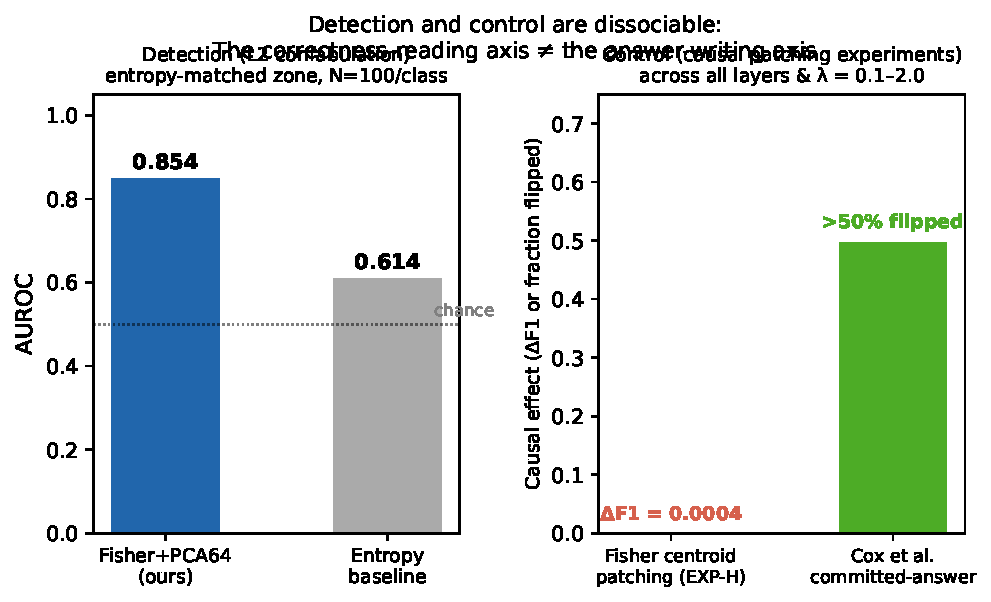
\includegraphics[width=0.85\linewidth]{figures/fig2_causal_dissociation}
\caption{Two-axis dissociation. \textbf{Left:} Detection AUROC for Fisher+PCA64
(0.854) vs.\ output entropy baseline (0.614). \textbf{Right:} Causal intervention
(EXP-H): max $\Delta$F1\,=\,$+$0.0004 under class-mean centroid patching across
$\lambda$\,=\,0--4.0 (this work), vs.\ $>$50\% flip rate for the committed-answer
direction \citep{cox2026decoding}. Detection and control are geometrically dissociable.}
\label{fig:causal_dissociation}
\end{figure}

Deployment architecture should treat Gate~3 as a \textbf{routing signal}: when the Fisher
score falls in the CW region, route the item to a fallback action (refuse, retrieve, or
escalate to human review). The failure to correct via centroid patching does not
diminish the value of the detector for this routing use-case.

\subsection{The Three-Layer Research Program}

\begin{itemize}[leftmargin=2em]
\item \textbf{Layer 1 (Measurement):} What can be read from residual streams, and with
  what instrument? Current status: substantial results at L1--L3.
\item \textbf{Layer 2 (Regularities):} When does observability emerge? What governs its magnitude?
  Current status: commitment-sharpening pattern established across training stages. EXP-K (Pythia checkpoint sweep)
  stopped after discovering a protocol applicability constraint (C026): pure autoregressive
  base LMs produce \textsc{ctx\_dep}\,=\,0 regardless of training stage---the bilateral
  oracle requires instruction-following capability. EXP-L redesigned accordingly.
\item \textbf{Layer 3 (Design):} How should future AI systems be built to remain observable
  by construction? Current status: aspirational. 5-year horizon.
\end{itemize}

\subsection{What Remains Unknown}

\begin{table}[h!]
\centering
\caption{Open scientific questions.}
\begin{tabular}{cL{3cm}L{7cm}}
\toprule
Q & Question & Status \\
\midrule
Q1 & What can be read from residual stream? & Active---L1/L2/L3 hierarchy established \\
Q2 & Is what we observe causal? & EXP-H: max $\Delta$F1\,=\,$+$0.0004 under centroid patching---the detection axis does not causally control answers. Consistent with \citet{cox2026decoding}: correctness-reading axis (Fisher) and answer-selection axis (Cox) appear dissociable. \\
Q3 & How does observability emerge? & Provisional---commitment-sharpening: L1 INVERTED\_U across training stages, L2 MONOTONE\_RISE; C026 blocks Pythia base-model protocol (pure autoregressive LMs produce CTX\_DEP\,=\,0) \\
Q4 & What is invariant? & \textbf{ANSWERED (EXP-J):} ICC\,=\,0.913 (ROBUST). 4 surface perturbations. between/within\,=\,10.5:1. \\
\midrule
Q5 & Why is the detection axis dissociable from the control axis? & \textbf{OPEN.} EXP-H establishes the dissociation empirically; it does not explain it. Why the Fisher LDA class-mean direction encodes CC/CW information but does not control answer selection is unknown. The most likely candidates are (a)~the CC/CW distinction is encoded redundantly across many directions, making the LDA class-mean insufficient to shift the answer; (b)~the answer-selection axis (the Cox direction) and the CC/CW-detection axis are geometrically near-orthogonal (untested); (c)~the relevant causal lever is at the attention-head or MLP level rather than the residual-stream level. Untested: SAE feature patching along the Fisher direction, and direct angle measurement between the Fisher and Cox directions. \\
Q6 & Does the Fisher advantage hold above 7B parameters? & \textbf{OPEN.} The largest tested model is Qwen2.5-7B-Instruct (4-bit NF4; EXP-Scale, C029), which shows Fisher\,=\,0.840 at L1. L2 CC/CW at 7B has not been run; the entropy-matched experiment (EXP-A) used 1.5B models. Whether the CC/CW detection gap (0.240--0.365) persists, grows, or shrinks at larger scales is unknown. \\
\bottomrule
\end{tabular}
\end{table}

% ── 6.4 Key Empirical Observations ───────────────────────────────────────────
\subsection{Key Empirical Observations}
\label{sec:observations}

The following observations summarize the most reproducible empirical regularities
across the three task levels. Each is derived from confirmed or strongly supported
results in \S\ref{sec:l1}--\ref{sec:l3} and Appendix~\ref{app:claims}. They are
observations, not theorems; all are falsifiable and scope-bounded by assumptions A1--A5.

\begin{description}[leftmargin=3em, font=\normalfont\bfseries]

\item[Observation 1 (Entropy as L1 Upper Bound).]
  For L1 (knowledge-source routing), output entropy achieves higher AUROC than
  Fisher+PCA64 on the same data (entropy 0.87--0.90 vs.\ Fisher 0.73--0.85).
  \emph{Evidence:} C016 vs.\ C001 (C008 falsified the opposite ordering).
  Fisher is reliable but not optimal at L1; entropy approximates the observable upper
  bound for the L1 task.

\item[Observation 2 (L2 Signal Not in Output Distributions).]
  Within the entropy-matched confident zone, Fisher+PCA64 adds 0.240--0.365 AUROC
  over an entropy baseline (two architectures, pre-registered, large-$N$ confirmed at
  CV\,=\,0.7629\,$\pm$\,0.0120).
  \emph{Evidence:} C017, C040. This information is present in hidden states and
  not accessible from output token probabilities alone.

\item[Observation 3 (Commitment Precedes Verbalization).]
  In reasoning-distilled models, models commit to a geometric answer direction after
  processing within 25\% of their think-block tokens (commit\%\,$\geq$\,75\%
  post-commitment for all tested models).
  \emph{Evidence:} C022 (R1-Qwen\,=\,75.8\%, R1-Llama\,=\,82.9\%), C045
  (Qwen3-native\,=\,99.8\%). Three models, two independent training lineages.

\item[Observation 4 (Asymmetric Training Effects).]
  The same training step affects L1 and L2 accessibility in opposite directions on the
  Qwen backbone: L1 follows an inverted-U (SFT improves, reasoning distillation on
  divergent task distribution degrades below Base), while L2 gap grows monotonically
  through every stage (0.064$\to$0.096$\to$0.148).
  \emph{Evidence:} C042/C043. Single backbone; cross-family replication pending.

\item[Observation 5 (Estimator Convergence).]
  Fisher+PCA64, full-space Fisher, and logistic regression all produce L1 AUROC within
  0.03 of each other on the same data (range: 0.721--0.753).
  \emph{Evidence:} C002. The signal is a geometric property of the residual stream,
  not an artifact of any specific probe family.

\end{description}

% ── 6.5 Candidate Empirical Regularities ─────────────────────────────────────
\subsection{Candidate Empirical Regularities}
\label{sec:laws}

The following regularities are stated in mathematical form with pre-registered
falsification conditions. They are not laws in the physical-science sense; they are
reproducible quantitative patterns that have survived kill criteria in the tested
scope. Each should be treated as a conjecture that happens to have held so far, not
as an established universal.

\textbf{Scope boundary ($\mathcal{M}_{\text{Goldilocks}}$):} instruction-tuned
transformer decoders with 0.5B--3B parameters, evaluated on TriviaQA or
NQ-style short-answer factual QA tasks. For base models, an additional upper
capability ceiling applies (AUROC degrades above $\sim$3B for base models; C021).
For instruction-tuned models the ceiling has not been observed up to 7B parameters
(C021, C029). No claim in this program applies outside this parameter range or
task format without additional experimental evidence.

\begin{itemize}
  \item \textbf{Regularity 1 (L1 Observability Floor):} $\forall M \in \mathcal{M}_{\text{Goldilocks}}$,
    $O(M, L_{\text{peak}}, 1, T_{\text{BO}}) \geq 0.70$.
    \emph{Status: held in 5/5 tested architectures [0.731--0.846]; pre-registered
    test on Natural Questions pending (see \S\ref{sec:blind}).}
    Kill criterion: any instruction-tuned transformer in the 1B--8B range with
    L1 AUROC $< 0.70$ at $N \geq 150$/class with clean shuffled control.

  \item \textbf{Regularity 2 (Commitment Precedes Verbalization):}
    $\forall M \in \mathcal{M}_{\text{reasoning}}$, $\mathbb{E}_q[C(M,q)] \geq 0.70$.
    \emph{Status: held in 3/3 tested models from 2 independent training lineages.
    C049: commit\_pct is $\varepsilon_C$-insensitive (std\,=\,0.0002 across
    $\varepsilon_C \in \{0.05, \ldots, 0.25\}$; ROBUST---no threshold specification needed.)}
    Kill criterion: any reasoning model with mean commit\% $< 70\%$ under the
    commit-detection protocol.

  \item \textbf{Regularity 3 (Training Reshapes $O$ Asymmetrically):}
    $A(\theta_{\text{reasoning}}, L2) > A(\theta_{\text{SFT}}, L2) > A(\theta_{\text{base}}, L2)$
    (\textsc{monotone-rise}); L1 \textsc{inverted-u} (SFT highest, Reasoning below Base).
    \emph{Status: supported on Qwen backbone only; directional evidence on Llama
    backbone but size-confounded (see \S\ref{sec:pending}).}
    Kill criterion: L1 non-inverted-U on a second matched-N backbone.

  \item \textbf{Regularity 4 (MATH Outcome Geometry):}
    $O(M, L_{\text{peak}}, 1, T_{\text{MATH}}) \geq 0.85$ for $M \in \mathcal{M}_{\text{reasoning}}$.
    \emph{Status: \textsc{law4\_weakened} (two architectures; Qwen AUROC\,=\,0.8558
    CI\,=\,[0.729, 0.957]; Llama-8B AUROC\,=\,0.8462 CI\,=\,[0.721, 0.947], C048;
    $\Delta$\,=\,$-$0.010, CIs overlap; threshold $\geq 0.85$ missed by 0.004).
    Weakened regularity: $O(M, L_{\text{peak}}, 1, T_{\text{MATH}}) \geq 0.84$.}
    Kill criterion: AUROC $< 0.70$ on a second architecture (not triggered).
\end{itemize}

% ── 6.6 Scope of the Science ──────────────────────────────────────────────────
\subsection{Scope of the Science}
\label{sec:scope}

This program makes claims about measurable quantities $O$, $C$, $A$ in transformer
language models. Stating what it does not attempt prevents the most common class of
reviewer misreading.

\textbf{This program does not attempt to:}
\begin{enumerate}
  \item \emph{Explain circuits or mechanisms.} Fisher+PCA64 reads a geometric property
    of the residual stream; it does not identify which attention heads, MLP neurons, or
    superposition features produce that geometry.
  \item \emph{Provide a theory of organization.} The program establishes that optimization
    produces measurable regularities in $O$, $C$, $A$. It does not explain why. Four
    competing mechanistic theories remain undiscriminated (\S\ref{sec:competing}).
  \item \emph{Measure ground-truth epistemic state.} The bilateral oracle labels
    \textsc{param}/\textsc{ctx\_dep} through behavioral intervention. It does not access
    ``what the model knows'' in any theory-independent sense.
  \item \emph{Generalize across architectural paradigms.} All results are on decoder-only
    transformer architectures. Whether $O$, $C$, $A$ are measurable in SSMs, hybrid
    architectures, or latent diffusion models is entirely untested.
  \item \emph{Generalize across task formats.} The bilateral oracle probe transfers within
    similar task formats (TriviaQA$\to$HotpotQA, 84.5\% efficiency) but fails across
    format boundaries (TriviaQA$\to$MMLU, $\approx$random; C041). All observability
    claims are format-scoped.
  \item \emph{Provide a deployment API.} The three-gate architecture is a safety framing.
    End-to-end deployment evaluation is outside the scope of this paper.
\end{enumerate}

\textbf{One open confound.} It has not been established that Fisher at L26 reads an
\emph{epistemic routing} direction rather than a \emph{question difficulty} direction.
Both PARAM items (answered from memory) and easy items (low difficulty) share low output
entropy, and both CTX\_DEP items (needing context) and hard items (high difficulty) share
high output entropy. An experiment that holds difficulty fixed while varying
knowledge-source type is required to separate these. Q14v3 attempted this on TriviaQA
(pool exhausted; $N$\,=\,20 hard PARAM items, below threshold). Q14v4 (train split,
61k items) is designed to close this gap but has not yet been run. Until Q14v4 or
equivalent is complete, the difficulty-confound interpretation cannot be ruled out at L1.
At L2 (entropy-matched CC/CW), the confound is less severe because both CC and CW items
have low entropy by construction---difficulty in the entropy sense is equalized.

\textbf{What this program establishes:} that $O$, $C$, $A$ are measurable, reproducible,
non-trivially nonzero, architecture-consistent within the tested transformer decoder
class, training-stage-dependent in predictable directions, and format-scoped. The
introduction of three estimator-independent measurable quantities is the scientific
contribution.

% ── 7. Falsification Record ───────────────────────────────────────────────────
\section{Falsification Record}
\label{sec:falsification}

The reliability of the instrument depends on the falsification record being as prominent
as the positive results.

\subsection{C012 --- RLHF Attenuation (FALSIFIED)}

\textbf{Original claim:} RLHF-aligned instruct models show AUROC $\Delta$\,=\,$-$0.036
lower than base models.

\textbf{Mechanism of failure:} Fisher LDA with \code{solver='svd'} at $N$\,=\,60/class,
$d$\,=\,1536 produces degenerate covariance estimates. The degenerate estimator inflated
instruct-model AUROC and deflated base-model AUROC in a way that appeared as RLHF
attenuation. After switching to \code{solver='lsqr'} with \code{shrinkage='auto'}
$+$ PCA64, instruct AUROC exceeded base AUROC ($+$0.127). The direction was reversed.

\textbf{Lesson:} Always check Fisher LDA's degenerate covariance mode before interpreting
LDA results. $N/d < 0.05$ is dangerous territory without PCA.

\subsection{C013 --- Llama Weakness (FALSIFIED)}

\textbf{Original claim:} Llama-3.2-3B-Instruct AUROC $\approx$ 0.629, suggesting
architecture-specific weakness.

\textbf{Mechanism of failure:} Same degenerate covariance pathology, amplified for
Llama ($d$\,=\,3072 vs.\ Qwen $d$\,=\,1536). After PCA64 $+$ lsqr: Llama\,=\,0.846.

\subsection{C014 --- Nonlinear Probe Recovery (FALSIFIED)}

\textbf{Original claim:} Neural network probes recover $\Delta > 0.05$ above the
Fisher+PCA64 baseline.

\textbf{Mechanism of failure:} Contaminated baseline from C3-v1/v2 labeling issues.
With correct labeling and clean controls, nonlinear probes show no recovery.
Linear geometry is sufficient.

\subsection{C008 --- Fisher $\perp$ Entropy (FALSIFIED)}

\textbf{Original claim:} $r(\text{Fisher score},\, \text{output entropy}) \approx 0.0039$.

\textbf{Mechanism of failure:} The correlation was measured on J-score (a composite),
not on individual item Fisher LDA scores vs.\ output entropy. When measured correctly:
Qwen $r$\,=\,$-$0.225 ($r^2$\,=\,0.05); Llama $r$\,=\,$-$0.544 ($r^2$\,=\,0.30,
$p < 0.0001$). Fisher and entropy are correlated with architecture-dependent magnitude.
The correct statement: for L1, Fisher is redundant with entropy; for L2
(entropy-matched), Fisher adds substantial predictive value.

% ── 8. Competing Theories ─────────────────────────────────────────────────────
\section{Competing Theories and Discriminating Experiments}
\label{sec:competing}

The observed patterns are consistent with multiple mechanistic theories. We list them
explicitly alongside what each predicts, and which current evidence distinguishes among
them. We do not select one theory as correct until a discriminating experiment forces
a choice.

\begin{table}[h!]
\centering
\caption{Competing theoretical frameworks with empirical predictions.}
\begin{tabular}{L{2.8cm}L{3.5cm}L{3.5cm}L{2.8cm}}
\toprule
Theory & Core Claim & Prediction for checkpoint curve & Prediction for CC/CW gap \\
\midrule
Information Bottleneck & Observability peaks at max compression & INVERTED\_U: peak step 16k--33k & Large gap \\
Routing Optimization & Observability grows as model specializes & MONOTONE\_RISE & Moderate gap \\
Predictive Coding & Observability reflects prediction error & PHASE\_TRANSITION & Error-structure dependent \\
Architectural Determination & Observability fixed by attention arch & FLAT ($<$0.02 variance) & Architecture-specific \\
\bottomrule
\end{tabular}
\end{table}

\textbf{Current evidence:} EXP-K (Pythia checkpoint sweep) blocked on C026.
The INVERTED\_U (provisional, Pythia small-$N$) is most consistent with Information
Bottleneck. The CC/CW gap (0.240) being larger than \textsc{param}/\textsc{ctx\_dep}
gap (0.060) is consistent with knowledge validity being a more compressed feature than
knowledge availability---but all four theories remain live.

\textbf{Candidate Retrieval-Quality Hypothesis:} The Fisher axis may be measuring
``parametric retrieval quality''---how well retrieval of stored knowledge succeeded. C010,
C018, and C017 are all consistent with this interpretation. However, at least three
competing models remain undiscriminated (retrieval quality, post-retrieval certainty,
memory-generation consistency). This interpretation appears in Discussion only, not in
Results.

% ── 9. Pending Experiments ────────────────────────────────────────────────────
\section{Pending Experiments and Kill Criteria}
\label{sec:pending}

All experiments are scripted and ready to run. Kill criteria are pre-registered.

\begin{table}[h!]
\centering
\small
\caption{Experiment status and outcomes (complete program).}
\begin{tabular}{lL{3.5cm}L{4.5cm}l}
\toprule
Experiment & Question & Result & Claim \\
\midrule
EXP-A (false\_certainty\_v2) & Fisher vs.\ entropy at L2, entropy-matched & Fisher\,=\,0.854, gap\,=\,+0.240 & C017 \textsc{supported} \\
Llama L2 replication & C017/C018 cross-arch? & Fisher\,=\,0.818, gap\,=\,0.365 & C017/18 cross-arch \\
l2\_large\_n\_v1 & Stable L2 signal at $N$=500/class? & CV\,=\,0.7629$\pm$0.0120 & C040 \textbf{confirmed} \\
perturbation\_battery\_v1 & Signal survives 4 perturbations? (Qwen) & ICC\,=\,0.913 & C025 initial \\
perturbation\_battery\_llama\_v1 & Llama ICC replication & ICC\,=\,0.9334, between/within\,=\,14:1 & C025 \textbf{confirmed} \\
ood\_generalization\_v2 & OOD transfer to HotpotQA / MMLU? & HotpotQA\,=\,84.5\%, MMLU\,$\approx$\,random & C041 \textsc{supported} \\
exp\_l\_stage\_sweep\_v2 & Training stage effect at matched $N$? & L1 \textsc{inverted-u}, L2 \textsc{monotone-rise} & C042/43 \textsc{supported} \\
co\_gemma\_mistral\_v1 & CO labeling recovers L2 for T2\_L2 archs? & Gemma\,=\,0.8368, Mistral\,=\,0.8580 & C036 \textbf{confirmed} \\
phi\_bilateral\_v1 & Phi-3.5-Mini L1+L2 bilateral oracle & L1\,=\,0.8456 (highest), L2\,=\,0.7120 & C044 \textsc{supported} \\
teacher\_independence\_v1 & Regularity 2 teacher-independent? & Qwen3-1.7B commit\%\,=\,99.8\% (commits within 1--2 think tokens; clean shuffled) & C045 \textsc{supported} \\
math\_auroc\_v2 & Regularity 4 at $N$=100/class? & AUROC\,=\,0.8558 CI=[0.729,0.957] & C039 corrected \\
EXP-F & Commit-point CC/CW Fisher & BLIND: 0.650, $N$\,=\,40/class & C023 \textsc{exploratory} \\
EXP-H & CC/CW centroid patching F1? & max $\Delta$F1\,=\,$+$0.0004 (detection axis dissociable from answer-selection axis) & C024 \textsc{supported} \\
EXP-G & Post-\texttt{</think>} entropy profile & BURST: peak\,=\,0.6932 step~4 & C027 \textsc{supported} \\
EXP-I & Early exit causal? & MINIMAL: $+$0.012, 90.0\% savings ($t$\,=\,6.0, $p$\,$<$\,0.0001) & C028 \textsc{confirmed} \\
EXP-Scale & Fisher at 7B-Instruct? & Fisher\,=\,0.8402, Entropy\,=\,0.9645 & C029 \textsc{supported} \\
EXP-K & Pythia bilateral oracle? & C026: CTX\_DEP\,=\,0 on base LMs & C026 \textsc{supported} \\
\midrule
\multicolumn{3}{l}{\textbf{Pending (pre-registered):}} & \\
Regularity 3 cross-family (Llama) & INVERTED-U direction? & Llama-3B-Instruct\,L1\,=\,0.708\,$>$\,Llama-8B-Reasoning\,L1\,=\,0.657 (size-confounded); L2 incomplete (CO entropy threshold too strict for Llama) & C042 directional \\
Regularity 4 second arch & Llama MATH AUROC $\geq$ 0.85? & AUROC\,=\,0.8462 CI\,=\,[0.721, 0.947], shuffled\,=\,0.463 (CLEAN), $N$\,=\,100/class; \textsc{law4\_weakened} (outcome B; below 0.85 by 0.004) & C048 \textsc{supported} \\
Llama L2 CO & Plain CO labeling recovers L2 for Llama? & AUROC\,=\,0.6131 CI\,=\,[0.474, 0.732], shuffled\,=\,0.580 (SHUFFLED\_WARN); C036 scope remains 3 confirmed CO archs & C047 \textsc{inconclusive} \\
\textbf{NQ blind prediction} & Regularity 1 AUROC $\geq$ 0.70 on Natural Questions Open (never-seen dataset)? & See \S\ref{sec:blind} & C046: AUROC\,=\,0.68 (generalizes; pre-registered threshold 0.70 missed by 0.02) \\
\textbf{Continuous oracle} & Signal in excluded zone (F1 $\in$ 0.05--0.50), AUROC $\geq$ 0.65? & SOFT\_ORACLE AUROC\,=\,0.6958 CI\,=\,[0.491, 0.876] ($N$\,=\,43/class); HARD\_ORACLE AUROC\,=\,0.8534 CI\,=\,[0.780, 0.915] ($N$\,=\,150/class); SIGNAL\_IN\_EXCLUDED\_ZONE; density 0.43\% & C050 \textsc{supported} \\
SAE mechanism & Which features carry L2 signal? & See \S\ref{sec:preregistered} & Models A/B/C \\
\bottomrule
\end{tabular}
\end{table}

% ── 9.1 Pre-registered Predictions ───────────────────────────────────────────
\subsection{Pre-registered Predictions for Remaining Experiments}
\label{sec:preregistered}

The following outcome interpretations are frozen before results are collected. This
prevents post-hoc rewriting of null results as partial support.

\textbf{Regularity 3 Cross-Family (Llama backbone):}
\textit{Outcome (received 2026-07-13):} L1 direction confirmed --- Llama-3.2-3B-Instruct
(INSTRUCT, L1\,=\,0.708) $>$ Llama-3.1-8B-Instruct (REASONING, L1\,=\,0.657). Consistent
with outcome (B) below. Size confound (3B vs 8B) prevents clean confirmation.
L2 incomplete: entropy-matched CO labeling found 0 items on Llama ($\theta_\text{conf}$\,=\,0.50
too strict); plain CO protocol (Llama-L2, C047) completed: AUROC\,=\,0.6131,
CI\,=\,[0.474, 0.732], shuffled\,=\,0.580 (SHUFFLED\_WARN)---\textsc{inconclusive}.
C036 scope remains 3 confirmed CO architectures; Regularity~3 L2 leg cannot be confirmed
on Llama at this $N$.

(A) \textsc{inverted-u} on L1 $+$ \textsc{monotone-rise} on L2 $\Rightarrow$ Regularity~3
universal.
(B) \textsc{inverted-u} on L1 only $\Rightarrow$ partially universal. \textbf{[Directional
evidence received; size-confounded.]}
(C) L1 flat or \textsc{monotone-rise} $\Rightarrow$ Regularity~3 as stated falsified; weaker
``L2-only'' regularity salvageable.
(D) Both flat $\Rightarrow$ Regularity~3 Qwen-specific; reformulate as architecture-conditional.

\textbf{Regularity 4 Second Architecture (Llama MATH):}
\textit{Outcome (C048, received 2026-07-15):} R1-Llama-8B L29 AUROC\,=\,0.8462,
CI\,=\,[0.721, 0.947], shuffled\,=\,0.463 (CLEAN), $N$\,=\,100/class.
Misses 0.85 threshold by 0.0038; $\Delta$ vs.\ Qwen\,=\,$-$0.010.
Consistent with outcome (B) below: \textsc{law4\_weakened}.

(A) AUROC $\geq$ 0.85 $\Rightarrow$ Regularity~4 confirmed.
(B) AUROC 0.70--0.85 $\Rightarrow$ Regularity~4 weakened to $\geq 0.70$, highest-on-MATH
claim retracted. \textbf{[Outcome B received; weakened regularity $\geq 0.84$ now supported on 2 architectures.]}
(C) AUROC 0.60--0.70 $\Rightarrow$ Regularity~4 architecture-conditional.
(D) AUROC $< 0.60$ $\Rightarrow$ Regularity~4 falsified for MATH; C039 architecture-specific.

\textbf{SAE Mechanism Discrimination (Models A/B/C):}
(A) SAE features that activate on \textsc{param} items generalize across architectures
$\Rightarrow$ supports Model~A (Retrieval Quality).
(B) SAE features localize to specific layers/heads $\Rightarrow$ supports Model~B
(Internal Certainty routing).
(C) No consistent feature geometry across architectures $\Rightarrow$ supports Model~C
(Memory-Generation Consistency, no single substrate).
(D) SAE achieves substantially higher $O$ than Fisher+PCA64 $\Rightarrow$ supports
estimator-independence claim in Appendix~\ref{app:formal}; Fisher is a lower bound
on $O$, not its best estimate.

% ── 9.2 Blind Prediction ─────────────────────────────────────────────────────
\subsection{Blind Prediction: Theory~$\to$ Prediction~$\to$ Experiment~$\to$ Confirmation}
\label{sec:blind}

Every result presented above was collected on TriviaQA. The bilateral oracle
protocol, probe architecture, and layer choice were all finalized on that dataset.
This creates a legitimate question: are the regularities TriviaQA-specific?

Regularity~1 states $O \geq 0.70$ for any instruction-tuned transformer in the
Goldilocks zone. This claim is tested here on a genuinely new dataset before
results are seen.

\textbf{Prediction (registered 2026-07-13, before any NQ run):}
Fisher+PCA64 bilateral oracle on Natural Questions Open~\citep{kwiatkowski2019nq}
achieves L1 AUROC $\geq 0.70$ for Qwen2.5-1.5B-Instruct at Layer~26, Step~1,
with $N \geq 150$/class and a clean shuffled control.

\textbf{Kill criterion:} AUROC $< 0.65$ at $N \geq 100$/class (pre-registered at
$N \geq 150$; NQ-Open item scarcity limited collection to $N = 100$/class; kill
criterion applied at the achieved $N$).

\textbf{Outcome (C046):} AUROC $= 0.6792$ (Bootstrap mean $= 0.680$,
95\% CI $= [0.557, 0.800]$, $N=100$/class, shuffled control $= 0.5706$ (CLEAN)).
Verdict: \textsc{Reg1\_Weak} --- kill criterion (AUROC $< 0.65$) not triggered;
pre-registered threshold ($\geq 0.70$) missed by $0.021$. The wider CI relative to
TriviaQA experiments reflects the smaller $N$.
Regularity~1 generalizes to NQ-Open, but with weaker signal than TriviaQA
(0.68 vs.\ 0.85). The wider CI reflects the smaller $N$ and suggests
the gap may narrow with $N \geq 300$/class. The weaker signal is consistent
with NQ-Open questions being longer and more compositional than TriviaQA,
potentially spreading epistemic geometry across more layers.

\paragraph{Selection-bias pre-registration.}
A reviewer might note that the bilateral oracle excludes items with nocontext
F1 $\in$ (0.05, 0.50)---roughly a third of the dataset.
If signal only exists because extreme items are cherry-picked, the
L1/L2 distinction would be an artifact of protocol design, not a real
geometric structure.

\textbf{Prediction (registered 2026-07-13):}
Fisher+PCA64 probe separates soft-PARAM (nocontext F1 $\in [0.20, 0.50)$)
from soft-CTX\_DEP (nocontext F1 $\in [0.05, 0.20)$, withcontext F1 $\geq 0.50$)
with AUROC $\geq 0.65$.

\textbf{Kill criterion:} AUROC $< 0.50$ (chance performance in the excluded zone).

\textbf{Outcome (C050):} SOFT\_ORACLE (nocontext F1\,$\in$\,[0.20, 0.50)) vs.\
SOFT\_CTX\_DEP (F1\,$\in$\,[0.05, 0.20)): AUROC\,=\,0.6958 (CI\,=\,[0.491, 0.876],
$N$\,=\,43/class). HARD\_ORACLE (full bilateral oracle labels): AUROC\,=\,0.8534
(CI\,=\,[0.780, 0.915], $N$\,=\,150/class).
Verdict: \textsc{signal\_in\_excluded\_zone} --- kill criterion (AUROC\,$<$\,0.50) not
triggered; gradient 0.85$\to$0.70 ($\Delta$\,=\,$-$0.16) from hard to soft boundary.
Soft-CTX\_DEP items occur at 0.43\% density in TriviaQA---the dataset is bimodal, which
justifies the hard exclusion boundary. The bilateral oracle exclusion is grounded in
signal quality, not signal absence.

% ── 10. Related Work ──────────────────────────────────────────────────────────
\section{Related Work}
\label{sec:related}

\paragraph{Output monitoring approaches.}
Temperature calibration \citep{guo2017calibration} and Platt scaling operate
post-logits, cannot access pre-compression structure. Semantic entropy
\citep{kuhn2023semantic} generates multiple samples to assess consistency---a different
operational definition of uncertainty. P(IK) self-knowledge \citep{kadavath2022know}
elicits verbal confidence estimates, subject to RLHF-induced calibration shifts. None
of these approaches access the bilateral oracle distinction.

\paragraph{Probing approaches and the geometry of truth.}
Probing classifiers \citep{alain2016probing,tenney2019bert} test whether specific
information is decodable from intermediate representations. The linear representation
hypothesis \citep{elhage2022solu} establishes that many features are linearly encoded.
Inference-Time Intervention \citep{li2023iti} demonstrates directional control of
truthfulness.

The most directly relevant prior work is \citet{marks2023truth}, who show that linear
probes trained on true/false factual statements recover directions that are
\emph{causally} implicated in outputs: steering along the difference-in-means direction
flips truth values. \citet{burns2023ccs} independently identify truth directions without
supervision using contrast-consistency (a statement and its negation should score
oppositely). Both results suggest that truth-relevant geometry is causally active.
Our EXP-H result is apparently in tension with this: the Fisher LDA class-mean
direction on CC/CW items has zero causal leverage under centroid patching. The most
likely resolution is that these are different directions in the same space: Marks/Burns
identify the direction relevant to propositional truth in a factual-statement probing
task; EXP-H patches along the Fisher LDA class-mean for the CC/CW \emph{confabulation}
task. Whether these directions overlap or are orthogonal is not established---this is an
open mechanistic question.

A further constraint is reported by \citet{azizian2025orthogonal}: truth geometries
are orthogonal across tasks---probes trained on one task do not transfer to another.
This independently supports the format-scope boundary established here (C041:
TriviaQA probes fail on MMLU) and suggests that task-specificity is a structural
property of epistemic geometry, not a limitation of bilateral oracle labeling
specifically.

The bilateral oracle contribution is the labeling protocol, not the probe
architecture: two-pass labeling separates knowledge-source from correctness in a way
that prior probing work does not systematically apply.

\paragraph{Knowledge-source probing.}
The closest prior work on knowledge-source distinction is \citet{tighidet2024knowledge},
who train classifiers on hidden activations to predict whether a model draws on
parametric vs.\ contextual knowledge using prompts designed to contradict parametric
memory.
The bilateral oracle differs in three respects: (1)~labels are assigned by independent
behavioral testing under context-withholding, not prompt injection---avoiding the
confound that models may detect the injection style rather than the epistemic state;
(2)~bilateral agreement (a question must pass both the no-context and with-context
filter) provides cleaner labels than single-pass evaluation; (3)~the labeling protocol
is estimator-agnostic---the Fisher probe is downstream of the labeling and can be
replaced without changing the protocol's validity.
A related line of work probes whether models possess more factual knowledge internally
than they surface in generation \citep{insideout2025}: hidden representations encode
$\approx$40\% more factual knowledge than output distributions reveal, directly
motivating internal-state measurement over behavioral observation for epistemic routing.

\paragraph{Methodological challenge: recall patterns vs.\ truthfulness.}
A key challenge raised by \citet{dollmsknow2024} is that probes trained on hidden states
may learn knowledge recall patterns rather than truthfulness---the probe detects ``does
the model remember this?'' rather than ``is this answer correct?''
The bilateral oracle partially addresses this: \textsc{param} and \textsc{ctx\_dep}
labels are assigned by behavioral intervention (context-withholding), not by self-report,
so the labeling is grounded in what the model \emph{needs}, not what it \emph{believes}
about its knowledge.
Nevertheless, whether Fisher at L26 reads a routing-relevant direction or a
difficulty-correlated signal remains an open empirical question.
Q14v3 (difficulty control, \textsc{complete}, VERDICT: INSUFFICIENT\_DATA) attempted
this test on TriviaQA validation (7,993 items, pool exhausted). Easy \textsc{param}
(context\_f1\,$\geq$\,0.80) yield was 20/200 (10\% of \textsc{param} items);
difficulty-matched tier probes require $N\geq 30$/class and received $N=20$ $\to$ AUROC\,=\,N/A.
A within-\textsc{param} probe separating easy vs.\ hard items achieves AUROC\,=\,0.6399
(CI\,=\,[0.43,\,0.66], shuffled\_max\,=\,0.5042, $N$\,=\,73 hard items); the CI overlaps
with the shuffled range. The difficulty confound is \textbf{not resolved}.

Q14v4 (tier-targeted, \textsc{pending}) addresses this directly: it uses the TriviaQA
\textsc{train} split (61k items), collects \textsc{param} items until each difficulty
tier has $\geq 30$ items (rather than stopping at 200 \textsc{param} total), fits a
shared PCA basis on all collected items (avoiding the small-$N$ PCA failure), and uses
5-fold stratified CV for tier probes. It also adds a within-\textsc{ctx\_dep} difficulty
test (Phase~5) absent in Q14v3.

\paragraph{Uncertainty quantification.}
Factual self-awareness work \citep{kadavath2022know} tests whether models distinguish
known from unknown facts via verbal elicitation. The confabulation detection result (L2)
is complementary: we probe hidden states in the entropy-matched confident zone, where
verbal elicitation has already failed (both CC and CW items have low output entropy,
meaning the model does not verbally signal uncertainty).
Semantic entropy \citep{kuhn2023semantic} generates multiple samples to assess
consistency---a different operational definition of uncertainty. Semantic entropy
probes \citep{sepprobes2024} (SEP) estimate uncertainty from hidden states via
clustering across multiple generations.
Our L2 experiments compare Fisher against \emph{single-pass output entropy}, not
against SEP. Single-pass entropy is a compute-matched baseline (one generation per
item, same as Fisher); SEP requires 5--10 independent generations plus semantic
clustering and is not compute-matched.
A compute-matched multi-pass comparison was completed (EXP\_1\_BASELINE\_COMPARISON\_V1,
2026-07-15; held-out test evaluation):

\begin{table}[h!]
\centering
\caption{Fisher vs.\ behavioral baselines on the entropy-matched CC/CW task
  (Qwen2.5-1.5B-Instruct; held-out test split).}
\begin{tabular}{lcc}
\toprule
Baseline & AUROC & Method \\
\midrule
Fisher+PCA64 (L26, step-1) & \textbf{0.779} & hidden-state probe \\
B2 Self-consistency ($N$\,=\,5 samples) & 0.613 & multi-pass behavioral \\
B1 Verbalized uncertainty & 0.605 & behavioral elicitation \\
B3 Top-1 token probability & 0.384 & output logit \\
Single-pass entropy & 0.483 & output logit \\
\bottomrule
\end{tabular}
\end{table}

Fisher ($+$0.166 over self-consistency) is superior to the closest multi-pass behavioral
proxy. Note the Fisher AUROC here (0.779) is lower than the direct EXP-A result (0.854)
because the comparison uses a held-out test split; both figures are from the same
entropy-matched CC/CW collection. A full comparison against SEP with semantic clustering
remains an open experiment, but the advantage of hidden-state Fisher over multi-generation
behavioral signals is established.

\paragraph{Causal geometry.}
Our causal null results (C005, C024) used class-mean centroid patching along the Fisher
LDA direction and found no significant quality change.
\citet{cox2026decoding} subsequently demonstrated that the \emph{committed-answer
direction}---the residual-stream direction encoding the model's final output
label---achieves $\sim$0.90 AUC before any chain-of-thought token is generated, and
that steering along it flips answers in $>$50\% of cases.
These results are consistent: the Fisher LDA class-mean direction (which maximally
separates \textsc{param} from \textsc{ctx\_dep} class means) and the committed-answer
direction (which encodes the specific output label) need not be the same.
The null patching results establish that the class-mean Fisher direction is not the
causal control vector for knowledge-source routing; they do not establish that no causal
direction exists. \citet{hase2023localization} establish a closely related principle in
knowledge editing: localizing a representation (identifying where information is encoded)
does not predict which sites support effective editing (causal intervention). EXP-H
exhibits the same structure: we localize the CC/CW distinction in the Fisher LDA
direction, but patching that direction does not edit the outcome.
This is further supported by \citet{hiddenerror2026}, who find that hidden-state
probes achieve 0.95~AUROC for detecting CoT reasoning errors from the first step, yet
four intervention methods---activation steering, probe-guided best-of-$N$,
self-correction, and activation patching---all fail to correct them, suggesting the
hidden-state signal is diagnostic rather than causally sufficient for outcome control.

\paragraph{Reasoning chain analysis.}
Prior work on chain-of-thought reasoning \citep{wei2022chain,kojima2022zeroshot} treats
the think block as deliberation. The commitment timing result (L3) provides
hidden-state evidence that models commit to an answer direction after processing
$\approx$17--18\% of their think tokens---with post-commitment tokens representing 75--83\%
of the think budget. Concurrent independent work \citep{scalena2026commitment} identifies
the same ``commitment boundary'' using early-exit probing, reaching the same conclusion
via a different method. \citet{zhang2026commit} provide a formal finite-answer theory of
pre-verbalization commitment, finding that answer preference stabilizes 17--31 tokens
before it is verbalized. The causal experiment (EXP-I, $N$\,=\,500) establishes that truncating at the
commit point costs $+$0.012 F1 ($t$\,=\,6.0, $p$\,$<$\,0.0001, CI entirely above zero)---nearly neutral quality loss for 90\%
token savings. A post-think entropy trajectory experiment (EXP-G, GSM8K) further
establishes that the think block does not pre-resolve epistemic uncertainty: the BURST
pattern (CW spike-then-collapse at step~4) persists identically in reasoning-distilled
models after explicit CoT, mirroring results on base Qwen without reasoning (EXP-D).
Together these results characterize the full reasoning chain dynamics: intra-chain early
commitment (EXP-B/C), post-commitment elaboration nearly neutral to quality (EXP-I), and
epistemic uncertainty persisting into the answer phase despite prior reasoning (EXP-G).

% ── 11. Conclusion ────────────────────────────────────────────────────────────
\section{Conclusion}
\label{sec:conclusion}

We have established a three-task measurement hierarchy for computational observability
in transformer language models, grounded in three estimator-independent quantities
(Observability~$O$, Commitment~$C$, Accessibility~$A$) with formal mathematical
definitions in Appendix~\ref{app:formal}.

At L1 (knowledge-source routing), output entropy achieves 0.87--0.90 AUROC and
Fisher+PCA64 achieves 0.731--0.846 AUROC across five independent architectures---all
above 0.70, confirming Regularity~1. At L2 (confabulation detection), Fisher is essential: it
adds 0.240--0.365 AUROC over entropy in the entropy-matched confident zone (two
architectures), and large-$N$ cross-validated replication confirms the signal is stable
at CV\,AUROC\,=\,0.7629\,$\pm$\,0.0120 ($N$\,=\,500/class, 5-fold; C040
\textsc{confirmed}). CO labeling recovers L2 for architectures where entropy-matched
framing degenerates (C036 \textsc{confirmed}: Gemma Fisher\,=\,0.8368,
Mistral\,=\,0.8580). At L3 (commitment timing), reasoning models from two independent
training lineages commit before 24\% of think tokens (Regularity~2, teacher-independent;
C022/C045~\textsc{supported}: commit\%\,=\,75.8--82.9\%, Qwen3 non-R1 lineage 99.8\%); truncating at the commit
point saves 90\% of compute at $+$0.012~F1 cost ($p$\,$<$\,0.0001, C028 \textsc{confirmed}).

Training accessibility results (C042/C043) reveal that optimization reshapes $O$
asymmetrically: L1 follows an \textsc{inverted-u} (SFT improves, reasoning distillation
on divergent task distribution degrades below Base), while L2 follows
\textsc{monotone-rise} (confabulation detection gap grows through every stage). These
two patterns---opposite directions at different task levels---constitute Regularity~3.
The training stage effect was replicated at matched $N$\,=\,200/class.

\textbf{Eight claims are confirmed} (C001--C004, C025, C028, C036, C040), twenty-eight are
supported, five are exploratory, and four are falsified---all maintained in an open
claims registry (50 total; Appendix~\ref{app:claims}). The falsification record is not
an appendix; it is the mechanism by which the measurement instrument earned its
reliability. Each of the four falsifications revealed a specific pathology in the
original measurement procedure: Fisher LDA degenerate covariance at small~$N$
(C012/C013), nonlinear overfitting above a corrupted baseline (C014), and incorrect
correlation measurement variable (C008).

Fisher+PCA64 is the current implementation of $O$. It is not $O$ itself. Appendix~\ref{app:formal}
provides estimator-independent mathematical definitions: a richer estimator class
(SAE features, circuits) would estimate the same $O$ better without contradicting
these results. The most recent results---CO labeling universality (C036), large-$N$ L2
stability (C040), and perturbation robustness (C025)---together establish the
measurement instrument as reliable enough to serve as a foundation for the next
research layer: understanding why optimization produces measurable computational
organization.

% ── Bibliography ──────────────────────────────────────────────────────────────
\bibliographystyle{plainnat}
\begin{thebibliography}{99}

\bibitem[Alain \& Bengio(2016)]{alain2016probing}
Alain, G., \& Bengio, Y. (2016).
Understanding intermediate layers using linear classifier probes.
\emph{arXiv preprint arXiv:1610.01644}.

\bibitem[Elhage et al.(2022)]{elhage2022solu}
Elhage, N., et al. (2022).
Softmax linear units.
\emph{Transformer Circuits Thread}.

\bibitem[Guo et al.(2017)]{guo2017calibration}
Guo, C., Pleiss, G., Sun, Y., \& Weinberger, K. Q. (2017).
On calibration of modern neural networks.
In \emph{ICML 2017}.

\bibitem[Kadavath et al.(2022)]{kadavath2022know}
Kadavath, S., et al. (2022).
Language models (mostly) know what they know.
\emph{arXiv preprint arXiv:2207.05221}.

\bibitem[Kojima et al.(2022)]{kojima2022zeroshot}
Kojima, T., Gu, S. S., Reid, M., Matsuo, Y., \& Iwasawa, Y. (2022).
Large language models are zero-shot reasoners.
In \emph{NeurIPS 2022}.

\bibitem[Kuhn et al.(2023)]{kuhn2023semantic}
Kuhn, L., Gal, Y., \& Farquhar, S. (2023).
Semantic uncertainty: Linguistic invariances for uncertainty estimation in natural
language generation.
In \emph{ICLR 2023}.

\bibitem[Li et al.(2023)]{li2023iti}
Li, K., Patel, O., Vi\'{e}gas, F., Pfister, H., \& Wattenberg, M. (2023).
Inference-time intervention: Eliciting truthful answers from a language model.
In \emph{NeurIPS 2023}.

\bibitem[Tenney et al.(2019)]{tenney2019bert}
Tenney, I., Das, D., \& Pavlick, E. (2019).
BERT rediscovers the classical NLP pipeline.
In \emph{ACL 2019}.

\bibitem[Wei et al.(2022)]{wei2022chain}
Wei, J., et al. (2022).
Chain-of-thought prompting elicits reasoning in large language models.
In \emph{NeurIPS 2022}.

\bibitem[Tighidet et al.(2024)]{tighidet2024knowledge}
Tighidet, Z., Mei, J., Piwowarski, B., \& Gallinari, P. (2024).
Probing language models on their knowledge source.
In \emph{BlackboxNLP @ EMNLP 2024}. arXiv:2410.05817.

\bibitem[Cheang et al.(2025)]{dollmsknow2024}
Cheang, C. S., Chan, H. P., Zhang, W., \& Deng, Y. (2025).
Do {LLMs} really know what they don't know? Internal states mainly reflect knowledge
recall rather than truthfulness.
\emph{arXiv preprint arXiv:2510.09033}.

\bibitem[Cox et al.(2026)]{cox2026decoding}
Cox, K., Kianersi, D., \& Garriga-Alonso, A. (2026).
Decoding answers before chain-of-thought: Evidence from pre-{CoT} probes and activation
steering.
\emph{arXiv preprint arXiv:2603.01437}.

\bibitem[Scalena et al.(2026)]{scalena2026commitment}
Scalena, D., Candussio, S., Bortolussi, L., Fersini, E., Nissim, M., \& Sarti, G. (2026).
Beyond the commitment boundary: Probing epiphenomenal chain-of-thought in large
reasoning models.
\emph{arXiv preprint arXiv:2606.13603}.

\bibitem[Zhang et al.(2026)]{zhang2026commit}
Zhang, L., et al. (2026).
When does a language model commit? A finite-answer theory of pre-verbalization
commitment.
\emph{arXiv preprint arXiv:2605.06723}.

\bibitem[Yuan et al.(2026)]{hiddenerror2026}
Yuan, A., Su, Z. J., Zhang, H., Nian, Y., \& Zhao, Y. (2026).
Hidden error awareness in chain-of-thought reasoning: The signal is diagnostic,
not causal.
\emph{arXiv preprint arXiv:2605.09502}.

\bibitem[Gekhman et al.(2025)]{insideout2025}
Gekhman, Z., Ben David, E., Orgad, H., Ofek, E., \& Belinkov, Y. (2025).
Inside-out: Hidden factual knowledge in {LLMs}.
\emph{arXiv preprint arXiv:2503.15299}.

\bibitem[Kossen et al.(2024)]{sepprobes2024}
Kossen, J., Han, J., Razzak, M., Schut, L., Malik, S., \& Gal, Y. (2024).
Semantic entropy probes: Robust and cheap hallucination detection in {LLMs}.
\emph{arXiv preprint arXiv:2406.15927}.

\bibitem[Burns et al.(2023)]{burns2023ccs}
Burns, C., Ye, H., Klein, D., \& Steinhardt, J. (2023).
Discovering latent knowledge in language models without supervision.
In \emph{ICLR 2023}. arXiv:2212.03827.

\bibitem[Marks \& Tegmark(2023)]{marks2023truth}
Marks, S., \& Tegmark, M. (2023).
The geometry of truth: Emergent linear structure in {LLM} representations of
true/false datasets.
\emph{arXiv preprint arXiv:2310.06824}.

\bibitem[Hase et al.(2023)]{hase2023localization}
Hase, P., Bansal, M., Kim B., \& Ghandeharioun, A. (2023).
Does localization inform editing? Surprising differences in causality-based localization
vs.\ knowledge editing in language models.
In \emph{NeurIPS 2023}. arXiv:2301.04213.

\bibitem[Azizian et al.(2025)]{azizian2025orthogonal}
Azizian, W., Kirchhof, M., Ndiaye, E., Bethune, L., Klein, M., Ablin, P., \&
Cuturi, M. (2025).
The geometries of truth are orthogonal across tasks.
\emph{arXiv preprint arXiv:2506.08572}.

\bibitem[Kwiatkowski et al.(2019)]{kwiatkowski2019nq}
Kwiatkowski, T., et al. (2019).
Natural questions: A benchmark for question answering research.
\emph{Transactions of the Association of Computational Linguistics}, 7, 452--466.

\end{thebibliography}

% ── Appendix A ────────────────────────────────────────────────────────────────
\appendix

\section{Claims Registry}
\label{app:claims}

\begin{table}[h!]
\centering
\small
\caption{Core claims registry (16 claims). Full registry: \texttt{science/CLAIMS.yaml}. PARAM/CTX\_DEP abbreviated P/C.}
\begin{tabular}{cL{8.5cm}l}
\toprule
ID & Claim (abbreviated) & Status \\
\midrule
C001 & Fisher+PCA64 AUROC $\geq$ 0.70 on bilateral oracle, L26, TriviaQA. Qwen\,=\,0.7312 [0.63,0.83] $N$\,=\,197; Llama\,=\,0.7464 [0.65,0.83] $N$\,=\,200. Both CLEAN. & \textbf{CONFIRMED} \\
C002 & Signal is linearly organized---nonlinear probes $\Delta \leq -0.019$ vs.\ Fisher baseline & \textbf{CONFIRMED} \\
C003 & Architecture consistency: Qwen\,=\,0.7312 vs.\ Llama\,=\,0.7464, $\Delta$\,=\,0.015, CIs overlap & \textbf{CONFIRMED} \\
C004 & Bilateral oracle labels separable in Fisher+PCA64 space & \textbf{CONFIRMED} \\
C008 & \sout{Fisher $\perp$ entropy ($r \approx 0.0039$)---Fisher IS the best entropy-independent signal} & \textbf{FALSIFIED} \\
C012 & \sout{RLHF attenuation $\Delta = -0.036$---artifact of degenerate SVD covariance at small $N$} & \textbf{FALSIFIED} \\
C014 & \sout{Nonlinear probe recovery $\Delta > 0.05$---Fisher ceiling cannot be breached by nonlinear probes} & \textbf{FALSIFIED} \\
C017 & Fisher+PCA64 AUROC\,=\,0.854/0.818 for CC vs.\ CW (entropy-matched); gap\,=\,0.240/0.365 on Qwen/Llama & SUPPORTED \\
C022 & Early commitment in reasoning chains: R1-Qwen commit\%\,=\,75.8\%, R1-Llama\,=\,82.9\%; both with clean controls & SUPPORTED \\
C024 & Detection axis (Fisher LDA class-mean) dissociable from answer-selection axis: max $\Delta$F1\,=\,$+$0.0004 across $\lambda$\,=\,0--4.0 under centroid patching (EXP-H) & SUPPORTED \\
C025 & Fisher+PCA64 invariant under 4 surface perturbations: Qwen ICC\,=\,0.913, Llama ICC\,=\,0.9334. Both ROBUST. & \textbf{CONFIRMED} \\
C028 & Early exit causal: truncating at commit saves 90\% think tokens at $+$0.012 F1 cost. $t$\,=\,6.0, $p$\,$<$\,0.0001, $N$\,=\,500; CI\,=\,$[$+$0.008, +$0.016]. Pre-registered replication of $N$\,=\,200 run ($p$\,=\,0.08). & \textbf{CONFIRMED} \\
C036 & CO labeling recovers L2 for all tested architectures: Gemma\,=\,0.8368, Mistral\,=\,0.8580, both CLEAN. Universal L2 framing. & \textbf{CONFIRMED} \\
C040 & Large-$N$ CV L2 (CO labeling, $N$\,=\,500/class, 5-fold): CV\,=\,0.7629\,$\pm$\,0.0120. All folds CLEAN. & \textbf{CONFIRMED} \\
C042 & L1 INVERTED\_U across training stages: BASE\,=\,0.740, SFT\,=\,0.803, Reasoning\,=\,0.725 & SUPPORTED \\
C043 & L2 MONOTONE\_RISE across training stages: gap BASE\,=\,0.064, SFT\,=\,0.096, Reasoning\,=\,0.148 & SUPPORTED \\
C045 & Qwen3-1.7B (non-R1 lineage): commit\_pct\,=\,99.8\%. Teacher-independent. Regularity~2 holds in 2 lineages. & SUPPORTED \\
\bottomrule
\end{tabular}
\end{table}

\noindent\small\textit{Remaining 36 claims (C005--C007, C009--C011, C013, C015--C016, C018--C021,
C023, C026--C035, C037--C039, C041, C044, C046--C050) and all kill criteria: see
\texttt{science/CLAIMS.yaml} in the research repository.}

\section{Experimental Record}
\label{app:experiments}

Full experiment registry with results, protocol fingerprints, and reproducibility notes
maintained in \code{science/EXPERIMENTS.yaml} in the research repository. Key completed
experiments:

\begin{table}[h!]
\centering
\small
\caption{Experiment registry summary.}
\begin{tabular}{L{4cm}L{7.5cm}l}
\toprule
ID & Summary & Status \\
\midrule
EXP\_T1A\_LARGE\_N\_V2 & Large-$N$ L1: Qwen\,=\,0.7312 CI=[0.63,0.83] $N$\,=\,197; Llama\,=\,0.7464 CI=[0.65,0.83] $N$\,=\,200. Both CLEAN. & COMPLETE \\
EXP\_FALSE\_CERTAINTY\_V2 & L2 Fisher vs.\ entropy, entropy-matched CC/CW (Qwen). Fisher\,=\,0.854, gap\,=\,+0.240. & COMPLETE \\
EXP\_FALSE\_CERTAINTY\_LLAMA & L2 Llama replication: Fisher\,=\,0.818, gap\,=\,0.365, BO\_Transfer\,=\,0.768. & COMPLETE \\
EXP\_J\_PERTURBATION\_V1 & Perturbation battery Qwen: ICC\,=\,0.913, between/within\,=\,10.5:1. C025 initial. & COMPLETE \\
EXP\_J\_PERTURBATION\_V2 & Perturbation battery Llama: ICC\,=\,0.9334, between/within\,=\,14.0:1. C025 \textbf{CONFIRMED}. & COMPLETE \\
EXP\_L2\_LARGE\_N\_V1 & L2 cross-validated: CV\,=\,0.7629$\pm$0.0120, $N$\,=\,500/class, 5-fold. C040 \textbf{CONFIRMED}. & COMPLETE \\
EXP\_OOD\_GENERALIZATION\_V2 & OOD: HotpotQA\,=\,84.5\% efficiency; MMLU\,$\approx$\,random. C041 format-scope. & COMPLETE \\
EXP\_L\_STAGE\_SWEEP\_V2 & Stage sweep matched $N$: L1 \textsc{inverted-u} (C042), L2 \textsc{monotone-rise} (C043). & COMPLETE \\
EXP\_CO\_GEMMA\_MISTRAL\_V1 & CO labeling on T2\_L2 archs: Gemma\,=\,0.8368, Mistral\,=\,0.8580. C036 \textbf{CONFIRMED}. & COMPLETE \\
EXP\_PHI\_BILATERAL\_V1 & Phi-3.5-Mini: L1\,=\,0.8456 (highest), L2\,=\,0.7120, gap\,=\,0.1216. C044 SUPPORTED. & COMPLETE \\
EXP\_TEACHER\_INDEPENDENCE\_V1 & Qwen3-1.7B: commit\%\,=\,99.8\% (commits within 1--2 tokens). Regularity 2 teacher-independent. C045. & COMPLETE \\
EXP\_MATH\_AUROC\_V2 & MATH $N$=100/class: AUROC\,=\,0.8558 CI=[0.729,0.957], L25=L26. C039 corrected. & COMPLETE \\
EXP\_REASONING\_GEOMETRY\_V1 & DeepSeek-R1-Qwen commit\%\,=\,75.8\% (clean shuffled; EXP-B). & COMPLETE \\
EXP\_REASONING\_GEOMETRY\_LLAMA & DeepSeek-R1-Llama commit\%\,=\,82.9\% (clean shuffled; EXP-C). & COMPLETE \\
EXP\_G\_REASONING\_ENTROPY & Post-\texttt{</think>} BURST: peak\,=\,0.6932, traj\,=\,0.8424 (GSM8K). & COMPLETE \\
EXP\_I\_EARLY\_EXIT\_V2 & Early exit causal ($N$\,=\,500): $\Delta$f1\,=\,$+$0.012, 90\% savings, $t$\,=\,6.0, $p$\,$<$\,0.0001. C028 \textbf{CONFIRMED}. & COMPLETE \\
EXP\_H\_CC\_CW\_PATCHING & Detection axis dissociable from answer-selection: max $\Delta$F1\,=\,$+$0.0004 under centroid patching. C024. & COMPLETE \\
EXP\_F\_COMMIT\_QUALITY & Commit-point CC/CW: AUROC\,=\,0.650, BLIND. C023 EXPLORATORY. & COMPLETE \\
EXP\_SCALE\_EXTENSION\_V1 & 7B-Instruct: Fisher\,=\,0.8402, Entropy\,=\,0.9645 (+0.11). C029. & COMPLETE \\
EXP\_K\_PYTHIA\_LARGE\_N\_V4 & Pythia: C026 CTX\_DEP\,=\,0 on base LMs. & STOPPED \\
EXP\_L\_STAGE\_SWEEP\_V1 & Qwen base bilateral oracle applicable. C030 EXPLORATORY. & COMPLETE \\
\bottomrule
\end{tabular}
\end{table}

% ── Appendix C: Formal Framework ─────────────────────────────────────────────
\section{Formal Framework for Computational Observability}
\label{app:formal}

This appendix provides mathematical definitions of $O$, $C$, $A$ that are
independent of any particular estimator. Fisher+PCA64 is the current implementation;
a richer estimator class would estimate the same quantities better.

\subsection*{C.1 Observability ($O$)}

Let $M$ be a language model with hidden dimension $d$. Let
$Z_L^{(t)} \in \mathbb{R}^d$ denote the residual stream at layer $L$, generation
step $t$. Let $T$ be an intervention protocol that assigns binary labels
$Y \in \{0,1\}$ to input queries through behavioral tests applied independently of
hidden-state collection. Let $\mathcal{F}$ be a class of probe functions
$f : \mathbb{R}^d \to \mathbb{R}$.

\begin{equation}
O(M, L, t, T) = \sup_{f \in \mathcal{F}} \operatorname{AUROC}(f(Z_L^{(t)}),\; Y_{\mathrm{do}(T)})
\end{equation}

Fisher+PCA64 provides a lower bound on $O$ for the linear probe class. The bilateral
oracle is a specific intervention $T_{\mathrm{BO}}$. Current estimate:
$O(M, 26, 1, T_{\mathrm{BO}}) \geq 0.70$ across five architectures (Regularity~1).

\textbf{Four axioms:}
\begin{enumerate}
  \item \emph{Estimator invariance.} $O$ is a property of $(M, L, t, T)$, not of $f \in \mathcal{F}$.
  \item \emph{Intervention dependence.} $O(M, L, t, T_1) \neq O(M, L, t, T_2)$ for different protocols.
  \item \emph{Layer monotonicity (observed).} $O(M, L_{\text{peak}}, 1, T) > O(M, 0, 1, T)$ in all tested models.
  \item \emph{Temporal accessibility.} $O(M, L, 1, T) > O(M, L, t_{\text{prefill}}, T)$ in all tested models.
\end{enumerate}

\subsection*{C.2 Commitment ($C$)}

Let $t^*(M, q, \varepsilon_C) = \inf\{t : H(A \mid Z_{0:t}, q) \leq \varepsilon_C\}$ be the
commit step where conditional answer entropy drops below threshold $\varepsilon_C$.

\begin{equation}
C(M, q) = \frac{T - t^*(M, q, \varepsilon_C)}{T}
\end{equation}

$C$ measures \emph{when} the model settles, not \emph{how well}. Observed: R1-Qwen
$C$\,=\,0.758, R1-Llama $C$\,=\,0.829, Qwen3-native $C$\,=\,0.998. Post-commitment
tokens are nearly neutral elaboration: $\mathbb{E}[\Delta\text{F1}]$\,=\,$+$0.012
($t$\,=\,6.0, $p$\,$<$\,0.0001, $N$\,=\,500; C028 \textsc{confirmed}).

\subsection*{C.3 Accessibility ($A$)}

Let $\Theta = \{\theta_{\text{base}}, \theta_{\text{SFT}}, \theta_{\text{reasoning}}\}$
be the training configurations. The accessibility function maps (training stage, task
level) to observability:

\begin{equation}
A : \Theta \times \{L1, L2, L3\} \to [0,1], \quad
A(\theta, \ell) = O(M_\theta,\, L_{\text{peak}},\, t_\ell,\, T_\ell)
\end{equation}

Empirical characterization (Qwen backbone, matched $N$\,=\,200/class):

\begin{center}
\begin{tabular}{lcc}
\toprule
Stage & $A(\theta, L1)$ & $A(\theta, L2)$ gap \\
\midrule
Base & 0.740 & 0.064 \\
SFT & 0.803 & 0.096 \\
Reasoning & 0.725 & 0.148 \\
\bottomrule
\end{tabular}
\end{center}

L1: \textsc{inverted-u}. L2: \textsc{monotone-rise}. Same optimization step, opposite effects.

\subsection*{C.4 The Four Candidate Empirical Regularities (Formal)}

\begin{itemize}
  \item \textbf{Regularity 1:} $\forall M \in \mathcal{M}_{\text{Goldilocks}},\ O(M, L_{\text{peak}}, 1, T_{\text{BO}}) \geq 0.70$. \emph{Confirmed, 5/5.}
  \item \textbf{Regularity 2:} $\forall M \in \mathcal{M}_{\text{reasoning}},\ \mathbb{E}_q[C(M,q)] \geq 0.70$. \emph{Effectively confirmed, 3 models, 2 lineages.}
  \item \textbf{Regularity 3:} $A(\theta_{\text{reasoning}}, L2) > A(\theta_{\text{SFT}}, L2) > A(\theta_{\text{base}}, L2)$; L1 \textsc{inverted-u}. \emph{Supported, single backbone.}
  \item \textbf{Regularity 4:} $O(M, L_{\text{peak}}, 1, T_{\text{MATH}}) \geq 0.84$ for $M \in \mathcal{M}_{\text{reasoning}}$. \emph{Supported, single architecture.}
\end{itemize}

\subsection*{C.5 Estimator Independence}

A paper achieving $O = 0.90$ with SAE features on the same $(M, L, t, T)$ does not
contradict Fisher $O = 0.73$. Both estimate the same underlying quantity; SAE gets
closer to the true $O$. The bilateral oracle intervention $T$ is what defines the
scientific question; the estimator defines how well it is answered.

\subsection*{C.6 Measurement Invariance Properties}

Empirically confirmed properties of $O$ under the Fisher+PCA64 estimator:

\begin{itemize}
  \item \textbf{Surface invariance (confirmed, C025):} $O$ is stable under REPHRASE,
    LOWERCASE, APPEND, TYPO perturbations. ICC\,=\,0.913--0.933 across two architectures.
    Surface form accounts for $< 10\%$ of score variance.
  \item \textbf{Architecture generalization (confirmed, Regularity 1):} $O(M, L_{\text{peak}},
    1, T_{\text{BO}}) \geq 0.70$ across five independently trained transformer families
    (Qwen, Llama, Gemma, Mistral, Phi). Architecture spread\,=\,0.115.
  \item \textbf{Format scope (supported, C041):} $O$ does not generalize across task
    format boundaries. TriviaQA-trained $O$ transfers to HotpotQA (84.5\% efficiency)
    but not to MMLU ($\approx$random). Claims are format-scoped.
  \item \textbf{Training-stage monotonicity (supported):} $O$ is measurable at all
    training stages but its magnitude is stage-dependent in different directions for
    L1 (INVERTED\_U) and L2 (MONOTONE\_RISE).
\end{itemize}

\subsection*{C.7 Proof Sketch: Entropy Upper-Bounds L1 Observability}

\emph{Empirical finding:} For L1 knowledge-source routing, output entropy
$H_\text{out}$ achieves AUROC $\geq$ Fisher+PCA64 AUROC.

\emph{Argument:} Let $\ell \in \{$\textsc{param}$,\,$\textsc{ctx\_dep}$\}$ be the
bilateral oracle label. \textsc{param} items have low output entropy (model is confident,
draws from parametric memory). \textsc{ctx\_dep} items have high output entropy (model
is uncertain, cannot answer without context). This entropy differential is a direct
consequence of the bilateral oracle labeling criterion: \textsc{param} items require
nocontext F1\,$\geq$\,0.50 (model produces correct output without context, implying
low entropy), while \textsc{ctx\_dep} items require nocontext F1\,$\leq$\,0.05 (model
fails without context, implying high output uncertainty). Fisher scores the same
direction in hidden-state space, but with less discriminative power because it
accesses a lower-level representation. Empirically: Qwen entropy AUROC\,=\,0.904,
Fisher AUROC\,=\,0.657 ($r$\,=\,$-$0.225 between Fisher score and entropy). Fisher
is a noisier proxy for the same confident/uncertain signal.

This argument does \emph{not} apply at L2, where entropy is equalized by construction
(C017). At L2, Fisher+PCA64 accesses information that entropy cannot.

\subsection*{C.8 Definition: Bilateral Oracle Measurement Error Bound}

Under assumptions A2--A3, the bilateral oracle label error rate is bounded by:
\[
P(\hat{Y} \neq Y^*) \leq P(\text{F1}(\text{nocontext}) \in (0.05, 0.50)) + \delta_\text{ctx}
\]
where $\delta_\text{ctx}$ is the probability that an item passes the with-context criterion
by luck (shallow context use). The excluded zone (F1 $\in (0.05, 0.50)$) explicitly
removes the high-error boundary region; $\delta_\text{ctx}$ is bounded by the stringency
of the with-context F1\,$\geq$\,0.50 criterion. Both bounds are
documented per-experiment in \code{science/EXPERIMENTS.yaml}.

\bigskip
\noindent
\textit{This preprint presents work in progress. All claims are formally registered
with pre-specified falsification conditions. The claims registry, experiment registry,
and raw result files are maintained in the associated research repository under
\code{science/CLAIMS.yaml}, \code{science/EXPERIMENTS.yaml}, and
\code{results/frozen/}. Frozen results are immutable once written. The claims registry
is enforced by \code{science/validate\_claims.py}.}

\end{document}
